\setcounter{footnote}{0}
\setcounter{section}{0}
\setcounter{ExNo}{0}
\begin{center}
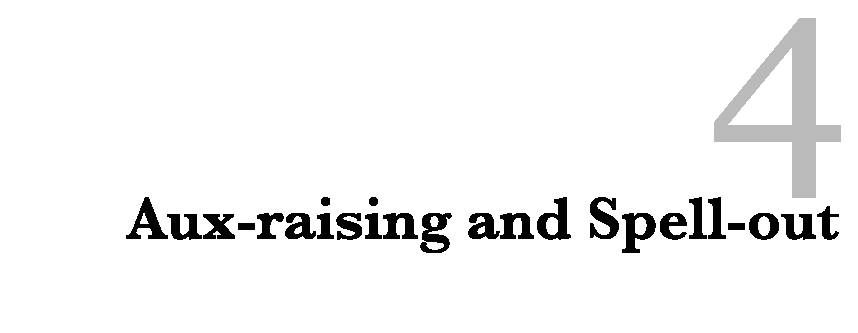
\includegraphics{chapter4.eps}
\end{center}
\section*{}
\addcontentsline{toc}{section}{\Large{Chapter 4: Aux-raising and Spell-out}}
\section{Introduction}
In the previous chapter I argued that tense-hopping occurs in Swedish as a feature-driven Lowering operation arising from the constraints imposed by the \textit{Phase Head Impenetrability Condition}, but that tense-hopping in English takes place in the PF representation as Local Dislocation. In this chapter, I explore these distinct models of tense-hopping further, paying specific attention to the asymmetry in the movement properties of auxiliary and main verbs in English. In Section 2, I propose a simplified, Minimalist analysis of this pattern that requires no look-ahead, no purely optional movement, nor a mixed lexicalist/non-lexicalist model of verbal morphology (cf.\ \citenop{lasnik1995}; see below), but rather relies on the ability to check morpho-syntactic features after Spell-out, i.e.\ on the PF branch, when the need arises. I claim that English, like Swedish, carries an uninterpretable V-feature on finite tense, and that auxiliary verbs in English raise to check this feature via narrow syntactic head-raising. However, narrow syntactic head-raising cannot check this feature in the case of main verbs due to the PHIC, as these, unlike auxiliaries, are not generated in the same phase as finite T in English, thus requiring the computational component to implement a tense-hopping strategy instead. Furthermore, extending the proposal of \citet{laka1990}, I posit that there is an ever-present syntactic projection in all clauses, $\Sigma$P, that houses negation and affirmation. I argue that the three-way distinction between negation (e.g.\ \textit{Bill didn't leave}), emphatic affirmation (e.g.\ \textit{Bill \textbf{did} leave}), and non-emphatic affirmation (e.g.\ \textit{Bill left}) is due to differences in the content of $\Sigma$P, which is never absent from the syntactic structure. Whereas Laka's Lowering analysis of the tense-hopping transformation prevented her from including $\Sigma$P in non-emphatic affirmation structures in English, the Local Dislocation analysis presented here not only allows for its inclusion in the syntax of all clauses, but also crucially relies on its presence, thus allowing for a more uniform syntactic structure across clause types. Moreover, I claim that it is the different syntactic positions that this $\Sigma$P occupies in Swedish vs.\ English that are solely responsible for the Lowering vs.\ Local Dislocation tense-hopping distinction between these two languages; namely, while finite T in both languages carries an uninterpretable V-feature, $\Sigma$P is an adjunct in Swedish, and so does not block Lowering of T, but is generated on the spine of the clause in English, and so disrupts the head-complement locality condition required for T-to-\textit{v} Lowering, thus requiring that finite T in English check its [-V] feature under Local Dislocation.

The perhaps most surprising claim here is that Local Dislocation---an operation occurring after Spell-out on the PF branch---may check uninterpretable morpho-syntactic features. I will argue that the capacity of the computational component to check uninterpretable features on the PF branch is a conceptual necessity from a strictly Minimalist perspective, under which there are but two true interfaces (i.e.\ pronunciation and interpretation).  Section 3 briefly explores the role of this projection further (e.g.\ the different patterns of negation cross-linguistically). Subsequent sections will address additional issues raised by the proposed model, including the interaction of late adjunction and Spell-out, and the mechanisms underlying instances of stem-allomorphy in verbal paradigms.


\section{Spell-out and feature-checking}\label{spellout_feature_check}
In this section, I address the consequences of the previous proposals for a theory of auxiliary-raising in English, investigating the syntactic role of the $\Sigma$P projection and the domain of feature-checking operations.

\subsection{Aux-raising}
Any theory of tense-hopping in English should also be able to account for the absence of tense-hopping in auxiliary constructions and, relatedly, the presence of auxiliary-raising. In this section, I develop a unified, feature-driven theory of auxiliary-raising, based in our previous analysis of tense-hopping transformations, that has profound implications for the interaction of Spell-out and feature-checking operations.

\subsubsection{Auxiliaries in English}
It is a well known fact that, although main verbs do not raise out of {\it v}P in English, auxiliary verbs raise to T. The examples in \Next[a-b] show that the auxiliary {\it have} appears to the left of the {\it v}P-adjunct and negation. The examples in \Next[c-d] illustrate that the auxiliary has adjoined to T before T-to-C interrogative movement is evaluated.\footnote{See \S\ref{Se_aux_sec} for the status of auxiliary verbs in Swedish.}

\singlespacing
\begin{quote}
\ex.
\a. John \underline{has} {\bf often} forgotten the address.
\b. John \underline{has} {\bf not} forgotten the address.
\c. \underline{Has} John forgotten the address?
\d. *Does John \underline{have} forgotten the address?

\end{quote}
\onehalfspacing
These data indicate that auxiliary verbs in English are not subject to tense-hopping, unlike main verbs. Several analyses have been proposed to explain this asymmetry between main and auxiliary verbs. For example, \citet{chomsky1993} adopts a purely lexicalist view of all verbal morphology, arguing that all inflected verbs raise at some point in the derivation. The difference between a verb-raising language and a tense-hopping language is that verbs raise overtly in verb-raising languages (i.e.\ the V-features of Agr are strong) and that verbs raise covertly in tense-hopping languages (i.e.\ the V-features of Agr are weak). Chomsky argues that auxiliary verbs in English must raise overtly, however. He posits that the auxiliaries {\it have} and {\it be} are semantically vacuous, and thus they are invisible to operations at LF (i.e.\ covert operations). Therefore, if the auxiliaries do not raise overtly, they cannot raise at all, leaving the V-features of Agr unchecked. I, of course, do not adopt this analysis here, given that we are working within the framework of Distributed Morphology. I will point out, however, that even under lexicalist Minimalist assumptions, this theory raises some questions. For example, the overt derivational component must somehow be cognizant of the fact that auxiliary verbs will be unable to move at LF, and so it moves them overtly, assuming that overt movement is evaluated before covert movement (e.g., as in \citenop{nissenbaum2000} and many others). While this is not an implausible scenario, it does require a perhaps undesirable derivational look-ahead in which overt operations can foresee the impossibility of later covert movements. More important, however, is the fact that it weakens the dichotomy of strong vs.\ weak features in that an overt movement may be induced by both, depending on the semantic interpretability of the moving elements.

Taking into consideration similar problematic aspects of a purely lexicalist account of this asymmetry, \citet{lasnik1995} proposes a hybrid lexicalist/non-lexicalist model of English verbal morphology. In particular, he argues that all verbs that raise cross-linguistically are fully inflected in the lexicon and carry uninterpretable features, whereas verbs that do not raise are uninflected in the lexicon and carry no uninterpretable features. Thus, for example, all French verbs and English auxiliary verbs come into the syntax with all of their inflectional features, but English main verbs enter the syntax in their bare form. Correspondingly, there are two types of INFL cross-linguistically (and even within a single language); one is a set of abstract features and the other is a morpho-phonological affix. These correspond, respectively, to verb-raising constructions and tense-hopping constructions. For example, in English the featural INFL only enters the syntactic derivation when it scopes over a fully inflected verb (i.e.\ an auxiliary) and raises that verb, checking the features of both the featural INFL and the inflected verb; the INFL that is a morpho-phonological affix only merges into the derivation when it scopes over an uninflected verb (neither of which carry uninterpretable features), and will undergo tense-hopping under PF string-adjacency via a mechanism similar to our Local Dislocation analysis above. A consequence of this model is that if a featural INFL scoped over an uninflected verb, the derivation would crash, as INFL's features would go unchecked; likewise, if an affixal INFL scoped over an inflected verb, the features of the verb would go unchecked, and the derivation would crash. Thus, only derivations that contain both a featural INFL and an inflected verb (e.g.\ a finite auxiliary construction), or both an affixal INFL and a bare verb (e.g.\ a finite main verb construction), will converge.

While I clearly believe that \citeauthor{lasnik1995}'s analysis of tense-hopping in main verbs in English is on the right track, an immediate problem with this model, and one that \citeauthor{lasnik1995} recognizes, is that it cannot easily account for the tense-hopping facts in Swedish. Swedish verbs do not raise independently to T (suggesting they are like English main verbs, i.e.\ bare), yet they also show signs of having a featural INFL (e.g.\ as evidenced by the fact that, like in French, T-to-C movement targets the main verb, as illustrated earlier). While I won't go into the details of his solution, \citeauthor{lasnik1995} suggests that Swedish verbs, like French verbs and English auxiliaries, come into the derivation fully inflected, but that the features on the featural INFL are weak in Swedish, whereas they are strong in English and French. However, with this claim, I believe that this system does not take us much further beyond \posscitet{chomsky1993} original claims.

Furthermore, the fact that \citeauthor{lasnik1995}'s model crucially relies on a hybrid lexicalist/non-lexicalist model of inflection is directly in opposition to the strict non-lexicalist model of Distributed Morphology advocated in this thesis. In the following sections, I propose that a simple adjustment to our view of where auxiliary verbs are merged in the narrow syntax allows us to derive a purely non-lexicalist model of auxiliary-raising in English under the model of syntactic derivation proposed in Chapter 3. Furthermore, I argue that we can do so without positing multiple lexical entries for individual morphemes, in addition to allowing for the exact same feature specifications for main and auxiliary verbs in English.

\subsubsection{A simplified approach to English aux-raising}
First recall that I make the default Minimalist assumption that all syntactic transformations are feature-driven. Thus, narrow syntactic raising of auxiliary verbs should be no exception, like under \posscitet{lasnik1995} theory. Let us furthermore assume, for the sake of argument, that auxiliary verbs are structurally and featurally identical to all other verbs; i.e., like lexical verbs, auxiliary verbs can be decomposed into a V head and a (possibly defective, i.e.\ non-argument-introducing) {\it v} head.\footnote{Note that this will ultimately not be crucial to our analysis of English auxiliaries, but it does allow for structural uniformity among all verb types.} Finally, let us assume that auxiliary-raising occurs due to an uninterpretable feature on finite T, rather than an uninterpretable feature on the auxiliary itself (contra \citenop{omaki2008}). Note that when auxiliaries are stacked, as shown in \Next[a], only one auxiliary obligatorily moves to T, thus indicating that it is not a lexically specified uninterpretable feature on the auxiliary that motivates movement, as this feature would go unchecked on the lower auxiliary in such a construction, predicting a derivational crash.\footnote{\citet{lasnik1995} and \citet{omaki2008} must posit multiple lexical entries for auxiliaries; one that contains uninterpretable features and undergoes raising and another that contains no uninterpretable features and does not undergo raising (or, alternatively, inflected and non-inflected lexical entries for auxiliaries). However, I maintain that auxiliaries, like main verbs, carry no uninterpretable features themselves, and that there is only one lexical entry per morpheme.} Furthermore, as shown in \Next[b], when T does not contain a finite bound morpheme, auxiliary-raising does not occur.

\singlespacing
\begin{quote}
\ex.
\a. Bill has not been sleeping well.
\b. Sue will not have finished the book by tomorrow.\footnotemark 

\end{quote}
\footnotetext{There is also the availability of constituent, rather than sentential, negation here; e.g.\ {\it Bill has been [not [sleeping well]]}, {\it Sue will have [not [finished the book]]}. However, these require more focus on {\it not} than do the examples in \Last. I take this distinction to be one in the syntactic position of negation, rather than the position of the auxiliaries. See \S\ref{sigma_aux_sec}.}
\onehalfspacing 
I will additionally assume that the feature on finite T in English is consistent. In other words, contra \citet{lasnik1995}, any finite tense morpheme consistently carries the same uninterpretable feature, and there is no corresponding version of the morpheme in the lexicon that lacks this feature, thus further minimizing the internal complexity of the lexicon. Taking these assumptions into account, we are again faced with two theoretical possibilities to derive auxiliary-raising; finite English T bears either a [-{\it v}] feature or a [-V] feature. Not surprisingly, we can immediately rule out a [-{\it v}] feature on English finite T. As argued earlier, any language that carries [-{\it v}] on finite T will exhibit verb-raising of all matrix verbs, which is clearly not the case in English. I thus argue that finite T in English, like finite T in Swedish, carries a [-V] feature. It is this feature that drives auxiliary-raising. This therefore creates a uniformity in the feature specifications of INFL in tense-hopping languages, further supporting the model of the {\it Rich Agreement Hypothesis} in Section \ref{rich_agr_sec} of Chapter 3 (i.e.\ languages that lack rich verbal inflection carry a [-V] feature on T). Before I present an argument as to why the same feature specification on T produces different tense-hopping patterns in English and Swedish, I will first show how a [-V] feature on finite English T is satisfied by verb-raising instead of tense-lowering in the presence of an auxiliary.

\subsubsection{Auxiliaries as functional elements}
I previously argued that a [-V] feature on Swedish T causes Lowering of T to the {\it v} head of its phase complement due to the PHIC. Thus, this same structural scenario cannot hold for auxiliary-raising in English. In other words, the structure for English auxiliary constructions cannot be the following, where finite T carrying a [-V] feature takes a {\it v}P phase complement whose head consists of a {\it v}$^{0}$ with an embedded V auxiliary (box indicates the Spell-out domain):

\singlespacing
\begin{quote}
\ex. \Tree
[.TP T\raisebox{-3pt}{\footnotesize{[-V]}}\\\{\sc{fin}\}
[.{\it v}P [.{\it v}\0 V\0\\AUX {\it v} ]
[.VP \sout{V} \qroof{main verb}.{\it v}P
].VP ].{\it v}P !{\qframesubtree} ]

\end{quote}
\onehalfspacing
Therefore, assuming that the PHIC holds, it must the case that auxiliaries either have a different structure from \Last or are merged in a different position from that illustrated in \Last, since finite T does not lower to auxiliary verbs. We are again faced with two possibilities; either 1) the auxiliary is merged in the lower phase (i.e.\ it is included in the lexical phase sub-array along with the lexical verb) but projects only a VP, and not a {\it v}P, or 2) the auxiliary is merged in the same phase as T (i.e.\ it is included in the functional sub-array), in which case it could project either just a VP or a higher {\it v}P and still be targetable for movement to T, since the PHIC would not apply. Each of these options is illustrated below (see later discussion for the syntactic position of Asp in auxiliary constructions):

\singlespacing
\begin{minipage}{5.5in}
\begin{quote}
\ex. {\it Option 1: AUX merged in lexical domain/phase and projects only a VP}\\
\Tree
[.TP T\raisebox{-3pt}{\footnotesize{[-V]}}\\\{\sc{fin}\}
[.VP V\0\\AUX \qroof{main verb}.{\it v}P
].VP !{\qframesubtree} ]

\end{quote}
\end{minipage}\\\\
\onehalfspacing
Here, similar to {\it v}-to-T\raisebox{-3pt}{\footnotesize{[-{\it v}]}} verb-raising, the PHIC does not prevent narrow syntactic raising of the auxiliary V to finite T, since V$^{0}$ is the highest head in the Spell-out domain, and so it is accessible to the higher T head; i.e.\ the feature at the edge of this phase is the V-feature of the auxiliary.

\singlespacing
\begin{minipage}{5.5in}
\begin{quote}
\ex. {\it Option 2a: AUX merged in functional domain/phase and projects only a VP}\\
\Tree
[.TP T\raisebox{-3pt}{\footnotesize{[-V]}}\\\{\sc{fin}\}
[.VP V\0\\AUX \qroof{main verb}.{\it v}P !{\qframesubtree}
].VP ]

\end{quote}
\end{minipage}\\\\
\onehalfspacing
In \Last, the auxiliary is included in the sub-array of functional elements. Therefore, when the auxiliary merges, it is itself the trigger for Spell-out of the functional elements in the lower {\it v}P, since I argue that a phase is triggered for Spell-out when a head from a separate sub-array is merged into the derivation (but see the upcoming discussion on the position of Asp in auxiliary constructions). In this way, since AUX and T are found in the same Spell-out domain, the V-feature of AUX is visible to T for narrow syntactic raising.

\singlespacing
\begin{minipage}{5.5in}
\begin{quote}
\ex. {\it Option 2b: AUX merged in functional domain/phase and projects a {\it v}P}\\
\Tree
[.TP T\raisebox{-3pt}{\footnotesize{[-V]}}\\\{\sc{fin}\}
[.{\it v}P [.{\it v}\0 V\0\\AUX {\it v} ]
[.VP \sout{V} \qroof{main verb}.{\it v}P !{\qframesubtree} 
].VP ].{\it v}P ]

\end{quote}
\end{minipage}\\\\
\onehalfspacing
Option 2b in \Last is similar to Option 2a in \LLast. Here, also, since the auxiliary is contained in the same Spell-out domain as T, narrow syntactic raising is predicted to be possible to check the [-V] feature on T; the fact that V$^{0}$ is embedded in {\it v}$^{0}$ does not hinder the feature-checking process within a Spell-out domain, since the PHIC is not a consideration when evaluating phase-internal head movement. For our purposes, Options 2a and 2b are equivalent, since they make no different empirical or theoretical predictions within the current model. However, since Option 2b allows for a greater uniformity between the structure of main and auxiliary verbs, we will adopt this as the working alternative to Option 1.\footnote{Several main verbs also project a ``defective'' {\it v}; e.g. unaccusatives. Therefore, Option 2b allows for a linguistic model in which all verbs---main and auxiliary---project a {\it v}, though the properties of that {\it v} may vary.}

As mentioned previously, all of the above options can potentially account for the pattern of auxiliary-raising in English. However, Option 1, in which the auxiliary verb is generated within the lexical domain/phase, creates a problem for progressive (and, as I will argue later, perfective) aspectual morphology. Assuming that the progressive {\it -ing} morpheme in English is generated in its own syntactic head, it is necessarily the case that it is generated below the auxiliary. Otherwise, auxiliary-raising would drag along this morpheme due to the Head Movement Constraint \citep{travis1984}. The basic structure must therefore be that in \Next[a], rather than \Next[b] (here I label the auxiliary verb projection simply as AuxP, since it is not the structure of the auxiliary projection itself we are concerned with, but rather its position with respect to T and the progressive morpheme).

\singlespacing
\begin{quote}
\begin{samepage}
\q\lb{prog_asp_tree}{\textit{Progressive aspect; e.g.\ `Is Bill running?'}}

\begin{quote}
\begin{enumerate}
\qtreecenterfalse
\item[(a)]
\qtreepadding1pt\small{\Tree
[.TP T\raisebox{-3pt}{\footnotesize{[-V]}}\\\{\sc{fin}\} [.AuxP Aux\raisebox{-3pt}{\footnotesize{[V]}}\\\{{\it be}\} [.AspP Asp\\\{{\it -ing}\} \qroof{$\ldots$}.{\it v}P ].AspP ].AuxP ]}
\hskip .05in \normalsize{(b)}
\qtreepadding3pt\small{\Tree
[.*TP T\raisebox{-3pt}{\footnotesize{[-V]}}\\\{\sc{fin}\}
[.AspP Asp\\\{{\it -ing}\}
[.AuxP Aux\raisebox{-3pt}{\footnotesize{[V]}}\\\{{\it be}\} \qroof{$\ldots$}.{\it v}P
].AuxP ].AspP ]}\\
\end{enumerate}
\qtreecentertrue
\end{quote}
\end{samepage}
\end{quote}
\onehalfspacing
Only the general structure in \Last[a] can account for the Aux-to-T raising facts in English, since the progressive morpheme is not adjoined to the auxiliary, as would be required if Aux-to-T head movement occurred in \Last[b]. Recall, however, that progressive aspect is argued to be generated in Outer Aspect, just like the reduplicants in Tagalog and Ndebele (see Chapter 2, \S\ref{non-vary_sec}.2). That is, under the current analysis, Outer Aspect/progressive is merged in the functional domain, rather than the lexical domain, since it acts as a Spell-out trigger for the lexical domain, deriving Asp-to-{\it v} Lowering in Tagalog and Ndebele. Therefore, if Asp in \Last[a] is merged within the same Spell-out domain as T, it is necessarily the case that the auxiliary is also merged in this functional domain, rather than in the lexical domain with the main verb. An alternative is that the structure in \Last[a] is correct, but both the auxiliary verb and the progressive morpheme are merged in the lower/lexical phase (i.e.\ Outer Aspect is functional in Tagalog and Ndebele, but lexical in English); in this case, under Option 1, in which the auxiliary projects only a VP, the auxiliary would still be accessible to T for raising in \Last[a]. However, as we will see in \S\ref{aux_ellipsis_sec}, evidence from ellipsis suggests that the progressive {\it -ing} morpheme undergoes Lowering to the lexical verb, which, under the model proposed in this thesis, indicates that there is a phase boundary between progressive Asp and the {\it v}P in \Last[a]. Therefore, I adopt the model in which auxiliary verbs are merged in the same phase as the finite T that attracts them in auxiliary-raising. English auxiliaries are thus functional elements, and are included in the same phase sub-array as (outer) Asp, T, C, and, as we will see, $\Sigma$ (e.g.\ negation).

A distinction between auxiliaries as functional elements and main verbs as lexical elements allows for the verb-raising asymmetry in English. Since auxiliaries are generated in the same phase domain as finite T\raisebox{-3pt}{\footnotesize{[-V]}}, T can target the auxiliary for raising, as the default feature-checking transformation for elements in the same Spell-out domain is raising. However, since T\raisebox{-3pt}{\footnotesize{[-V]}} and lexical verbs are merged in different phase domains, the PHIC will apply and raising of the lexical verb embedded in {\it v}$^{0}$ is impossible to check T's [-V] feature (see below for how this feature gets checked in the absence of auxiliary-raising). However, this main vs.\ auxiliary verb distinction is not completely arbitrary. Not only does it account for the surface patterns of these two types of verbs, but it can also be motivated on semantic grounds. For example, recall that \citet{chomsky1993} argued that auxiliaries are ``semantically vacuous'', whereas main verbs are semantically contentful. I believe that this same distinction can be recast as ``English auxiliaries are functional, whereas English main verbs are lexical.'' Note that English auxiliaries, unlike English main verbs, encode strictly grammatical properties, e.g.\ progressive {\it be} and perfective {\it have}.\footnote{This summation can easily be extended to copular forms of {\it be}, which generally take a predicative complement, though I will not address these constructions here.} That is, they do not introduce new semantic eventualities, or even provide information about the content of eventualities (i.e.\ what eventuality the clause expresses; e.g.\ walking, reading, eating, arriving, etc.), but rather add additional information about the grammatical aspect of an eventuality. In this way,---though they are, strictly speaking, verbs--, auxiliaries exhibit a close relationship with the functional Tense/Aspect/Mood properties of a clause. Therefore, I believe it is reasonable to suggest that they, as well, are included in the derivational sub-array that corresponds to functional elements in English.\footnote{But see \S\ref{Se_aux_sec} for the possibility of cross-linguistic variation with respect to which phase contains auxiliary verbs.}

\subsubsection{$\Sigma$P and the absence of tense-lowering in English}\label{sigma_sec}
In the preceding analysis, the auxiliary verb structurally intervenes between finite T and the lexical main verb. Therefore, it is not predicted that T would target the lexical main verb, since the V-feature on the auxiliary is the derivationally most recent instance of this feature when T merges and probes to check its [-V] feature.\footnote{See Chapter 3, fn. \ref{rel_min_fn} for a brief discussion of Relativized Minimality.} However, in the absence of an auxiliary, we might predict the following structure for an English clause:

\singlespacing
\begin{quote}
\ex. \Tree
[.TP T\raisebox{-3pt}{\footnotesize{[-V]}}
[.{\it v}P [.{\it v}\0 V\0\\\mbox{main verb} {\it v} ] $\ldots$
].{\it v}P !{\qframesubtree} ]


\end{quote}
\onehalfspacing
The structure in \Last is identical to that of Swedish tense-lowering. However, as argued previously, finite T in English does not undergo head-to-head Lowering to main verbs. Therefore, it cannot be the case that Swedish and English non-auxiliary clauses are both structurally and featurally identical.

Note that a crucial way in which English and Swedish differ is that negation is a blocker for tense-hopping in English, but not in Swedish:

\singlespacing
\begin{quote}
\ex. \a. I did \underline{not} read the book.
\bg. $\ldots$att jag \underline{inte} l\"{a}ste boken.\\
$\ldots$that I not read.\mbox{\sc{past}} book.\mbox{\sc{def}}\\
`$\ldots$that I did not read the book.'

\end{quote}
\onehalfspacing
A standard assumption regarding these facts---and one that I adopt here---is that negation in Swedish is an adjunct and that negation in English is generated on the spine of the derivation (i.e.\ it undergoes set-merge, by which it is a head that merges with a complement and projects, as opposed to the adjunct-merger operation of pair-merge; see \citenop{chomsky2001}) \citep{holmberg1993}. This produces the following two structures for English and Swedish negation, respectively (we will investigate the structure of the phrase housing negation below):\\

\begin{minipage}{5.5in}
\begin{quote}
\ex. {\it Negation in English and Swedish}

\begin{enumerate}
\qtreecenterfalse
\item[(a)]
\qtreepadding3pt\normalsize{\Tree
[.\normalsize{English}\\TP T\raisebox{-3pt}{\footnotesize{[-V]}}\\\{\sc{fin}\} [.NegP Neg\\\{{\it not}\} \qroof{$\ldots$}.{\it v}P ].NegP ]}
\hskip .3in \normalsize{(b)} \qtreepadding1pt\normalsize{\Tree
[.\normalsize{Swedish}\\TP T\raisebox{-3pt}{\footnotesize{[-V]}}\\\{\sc{fin}\} [.{\it v}P \qroof{\{{\it inte}\}}.NegP \qroof{$\ldots$}.{\it v}P ].{\it v}P ]}\\\\
\end{enumerate}
\qtreecentertrue
\end{quote}
\end{minipage}
\onehalfspacing
Under this structural model of negation, adjunct negation in Swedish \Last[b] will not block T-to-{\it v} Lowering, whether negation is merged early or late. Moreover, the English structure in \Last[a] precludes Lowering of T to the verb under our current model. Only a head that triggers Spell-out can undergo Lowering. In \Last[a], the Spell-out trigger is Neg, not T. Therefore, by the time T merges into the derivation in English, the V-feature on the main verb will have become impenetrable due to the PHIC, and thus it is inaccessible to T. We return to the status of [-V] on T shortly.

\citet{laka1990}, following \citet{chomsky1957}, observed that a similar blocking of tense-hopping occurs in emphatic affirmation structures in English; e.g.\ (where {\bf bold} indicates strong prosodic focus):

\singlespacing
\begin{quote} 
\ex.
\a. Bill \textbf{did} sell the car.
\b. *Bill did sell the car.

\end{quote}
\onehalfspacing
\citeauthor{laka1990} proposes that the {\it do}-support that arises in both negation and emphatic affirmation constructions is tightly related. Namely, she claims that both negation and emphatic affirmation are generated in the same syntactic projection, $\Sigma$P. Therefore, the basic structure of an English clause with {\it do}-support is the following (`\mbox{\sc{\textbf{aff}}}' = emphatic affirmation):

\singlespacing
\begin{quote}
\ex. \qtreepadding3pt\normalsize{\Tree
[.TP T\raisebox{-3pt}{\footnotesize{[-V]}}\\\{\sc{fin}\} [.$\Sigma$P $\Sigma$\\\mbox{\{\sc{neg/\textbf{aff}}\}} \qroof{$\ldots$}.{\it v}P ].$\Sigma$P ]}

\end{quote}
\onehalfspacing
Under \citeauthor{laka1990}'s analysis, $\Sigma$ acts as a structural intervener for Lowering of T to the verb in negation and emphatic affirmation constructions. This is also the claim of this thesis. In \Last, $\Sigma$ is the Spell-out trigger for {\it v}P, and so T will be unable to lower to the verb. However, given the ungrammaticality of \LLast[b], she assumes that $\Sigma$ is absent from the structure in non-emphatic affirmation constructions (i.e.\ standard declaratives). That is, since there does not appear to be a structural intervener for Lowering, as tense-hopping takes place here, a Lowering analysis of English tense-hopping requires that T take {\it v}P as its complement in \LLast[b], precluding the presence of $\Sigma$.

I propose that this is not the case, and that $\Sigma$ is present in all clauses. Under a Local Dislocation analysis of English tense-hopping, an intervening $\Sigma$ will be a blocker for tense-hopping only if it is phonologically contentful. However, regardless of its phonological status, an intervening $\Sigma$ head between finite T and {\it v}P will always block head-to-head Lowering, as desired. Under this model, the following is the structure for all clauses in English; the content of $\Sigma$ determines whether the clause is negative, emphatically affirmative, or non-emphatically affirmative (=`\mbox{\sc{aff}}'):\footnote{The distinction between emphatic and non-emphatic affirmation is merely the presence or absence of a focus feature. Focus features can be added to almost any syntactic constituent; e.g. \textit{John doesn't like \textbf{cats}, he likes \textbf{dogs}}. Therefore, an assumption implicit in the following discussion is that there is only one \{\mbox{\sc{aff}}\} morpheme, which is inherently phonologically null, but that a focus feature may be added to this morpheme, making it phonologically non-null, and thus a blocker for Local Dislocation.}

\singlespacing
\begin{quote}
\begin{minipage}{5in}
\ex. {\it Basic structure of all finite English clauses}\\\\
\qtreepadding3pt\normalsize{\Tree
[.TP T\raisebox{-3pt}{\footnotesize{[-V]}}\\\{\sc{fin}\} [.$\Sigma$P $\Sigma$\\\mbox{\{\sc{neg/\textbf{aff}/aff}\}} \qroof{$\ldots$}.{\it v}P ].$\Sigma$P ]}

\end{minipage}
\end{quote}
\onehalfspacing
Under \Last, Lowering of T to {\it v} is correctly predicted to always be impossible in English. However, only the phonologically contentful $\Sigma$ morphemes (e.g.\ {\it not} and the prosodic focus feature of \mbox{\sc{\textbf{aff}}}) will disrupt the morpho-phonological string-adjacency of finite T and the verb (modulo T-to-C and {\it v}P movement). The phonologically null \mbox{\sc{aff}} will be invisible in the morpho-phonological representation, and so string-adjacency of finite tense and the verb obtains; e.g.:\footnote{Since the phonological matrix of the non-emphatic affirmation morpheme, i.e.\ \mbox{\sc{aff}}, is null, the prosodic focus feature in emphatic affirmation must be phonologically realized on another morpho-phonological constituent, namely finite tense. I assume that the phonetic locus of a strong prosodic focus feature is determined at pronunciation. The focus feature on emphatic affirmation thus first acts as a phonological intervener for Local Dislocation, and is only later ``attached'' to the finite tense morpheme upon pronunciation. In this way, the morpho-phonological representation of a construction with emphatic affirmation would be the following when Local Dislocation is analyzed (where \mbox{\sc{\textbf{f}}} = focus feature): [-s $^{\wedge}$ \mbox{\sc{\textbf{f}}} $^{\wedge}$ read].}

\singlespacing
\begin{quote}
\ex. \mbox{[-s $^{\wedge}$} \mbox{\sc{aff}}\mbox{(=$\emptyset$) $^{\wedge}$ read]} = \mbox{[-s $^{\wedge}$ read]} $\rightarrow$ \mbox{[read+s]}


\end{quote}
\onehalfspacing
This model creates a syntactic uniformity among different clause types. Here, the distinction between negation, emphatic affirmation, and non-emphatic affirmation is not due to a difference in syntactic structure (i.e.\ the presence or absence of certain functional items in the numeration/derivation), but is rather the result of different specifications of the ever-present functional head $\Sigma$. Therefore, it is not the case that a non-emphatic affirmation clause is derived via the absence of a functional element, but, rather, all clause types are determined by the content of the $\Sigma$ head, which is always included in the numeration. Note that this is most likely the case for Swedish, as well (and, for that matter, perhaps all languages). As illustrated by the negation facts, $\Sigma$P in Swedish is an adjunct, and so no matter what the content of $\Sigma$, it will never block tense-lowering in Swedish.

In the case of auxiliaries in English, note that $\Sigma$ is a functional element, and so is merged in the same functional domain as auxiliaries and T. Therefore, $\Sigma$ will never block narrow syntactic raising of an auxiliary to T. We return to this issue in Section \ref{sigma_aux_sec}.

The consistent presence of a $\Sigma$P projection on the spine of the derivation in English correctly precludes T-to-{\it v} Lowering in all cases, and the phonological emptiness of the non-emphatic affirmation version of $\Sigma$ correctly allows for tense-hopping under Local Dislocation in standard English declarative clauses. However, there remains a serious issue to be addressed. Namely, in the absence of narrow syntactic auxiliary-raising, the [-V] feature on T is unable to be checked in the narrow syntax in English, given the unavailability of both verb-raising and tense-lowering. In the following section, I argue that this is exactly the case.

\subsection{Feature-checking after Spell-out}
Note that the [-V] feature on finite T in English \LLast can't be checked via narrow syntactic raising, since the only heads whose features are accessible in its probing domain are {\it v} and $\Sigma$, neither of which contains an accessible copy of the necessary interpretable V-feature. Therefore, under the proposed model, this [-V] feature will go unchecked in the narrow syntax in the absence of an auxiliary. Indeed, in the following sections, I propose that finite T in English non-auxiliary constructions does not check its [-V] feature in the narrow syntax, but rather checks this feature on the PF branch either as the result of Local Dislocation with the interpretable V-feature of the main verb or via {\it do}-support. I argue that this is possible under a strict definition of ``interface'' coupled with a Strong Minimalist Feature-checking Hypothesis (SMFH), which permits the checking of uninterpretable features on the PF branch after Spell-out.

\subsubsection{Local Dislocation as a ``feature-checking'' operation}
Recall that the PHIC states that features embedded within a complex phase head become unavailable for {\it narrow syntactic} feature-checking after Spell-out of that phase. Therefore, after Spell-out of {\it v}P, the only feature of the phase head that is still visible to the narrow syntax is the interpretable {\it v}-feature of the phase head. This is because all features of the phase have been transferred to the PF branch, and the narrow syntax can then only see the least embedded feature of that syntactic phase constituent (i.e.\ the ``edge'' feature).\footnote{Recall, however, that a cross-phasal narrow syntactic chain formed via Lowering allows a certain level of access to an impenetrable feature; see Chapter 3, \S\ref{loc_low_sec}. However, given the absence of tense-lowering in English, such a chain is not present.} All other features of the phase are still present in the PF representation after Spell-out, however. Under the derivational model proposed here, Spell-out triggering marks the embedded elements of a phase for transfer to PF, thus rendering them impenetrable in the narrow syntax. The transfer operation copies the narrow syntactic structure to the PF branch, where it is evaluated for phonological form. However, Spell-out transfer and Vocabulary Insertion do not erase morpho-syntactic features of morphemes at PF.\footnote{Indeed, given that Local Dislocation is (ostensibly) often sensitive to morpho-syntactic category (see \S\ref{cat_sens_sec}), the category feature of a morpheme must still be present after VI. This is also supported by the fact that assignment of prosody, which occurs very late, must also be able to see category information (e.g. {\it r\'{e}ject} (N) vs. {\it rej\'{e}ct} (V)).} That is, VI does not make these features ``impenetrable'' on the PF branch. Rather, operations on the PF branch add phonological form to those morphemes and linearize them with respect to one another, thus erasing the syntactic hierarchy, but not the morpho-syntactic features. In this way, Vocabulary Insertion is not a replacement operation, but truly a mapping operation in that it maps phonological form onto morpho-syntactic feature bundles, making them interpretable for the purposes of pronunciation, but does not delete the features of those bundles in the process. Therefore, I argue that the interpretable V-feature contained within the morpho-phonological representation of the complex {\it v} head is still available to check uninterpretable V-features on the PF branch; though the transfer operation makes the V-feature impenetrable in the narrow syntactic derivation, that feature remains active in the representation on the PF branch. Similarly, an uninterpretable feature that is transferred to the PF branch will remain uninterpretable after the transfer process, and so in order for the representation to converge, this feature must be checked before pronunciation via PF operations, or else the structure crashes (see below). For example, Spell-out of a structure corresponding to the sentence {\it John walked} will produce a morpho-phonological string at PF like the following (`$\surd$' indicates a checked feature):\footnote{Note that $\Sigma$P contains the non-emphatic affirmation morpheme in \Next, and so does not block Local Dislocation.}

\singlespacing
\begin{quote}
\ex. {\it John walked.}\\
\mbox{[John $^{\wedge}$ -ed\raisebox{-3pt}{\footnotesize{[-V]}} $^{\wedge}$ walk\raisebox{-3pt}{\footnotesize{[{\it +v}, +V]}}] $\rightarrow$ [John $^{\wedge}$ walk\raisebox{-3pt}{\footnotesize{[{\it +v}, +V]}}+-ed\raisebox{-3pt}{\footnotesize{[-V]$\surd$}}]}

\end{quote}
\onehalfspacing
Here, Local Dislocation of past tense and the verb checks the [-V] feature on finite T. I propose that the following occurs on the Vocabulary Insertion cycle on which phonology is mapped to the finite past tense morpheme:

\singlespacing
\begin{minipage}{5in}
\begin{itemize}
\item[1.] Phonological form is mapped to the \{\mbox{\sc{past}}, -V\} feature bundle, resulting in the form [-ed]\raisebox{-3pt}{\footnotesize{[-V]}}.
\item[2.] Since VI results in a bound inflectional morpheme, [-ed]\raisebox{-3pt}{\footnotesize{[-V]}} undergoes Local Dislocation with the verb, given that string-adjacency holds.
\item[3.] Since [-ed]\raisebox{-3pt}{\footnotesize{[-V]}} and the verb have now been fused into a single constituent, the [-V] feature on the tense morpheme is checked by virtue of its locality with the interpretable V-feature.

\end{itemize}
\end{minipage}\\\\\\
\onehalfspacing
Thus, Local Dislocation may result in feature-checking. I will address aspects of each of the above steps in turn. First, note that in Step 1 Vocabulary Insertion assigns phonological form to the \{\mbox{\sc{past}}\} feature, but leaves the [-V] feature intact; the [-V] feature here is not itself mapped to any phonological form. I take this to be a result of the {\it Subset Principle} \citep{halle_marantz1993}, stated below:

\singlespacing
\begin{minipage}{5.5in}
\begin{quote}
\ex. {\it Subset Principle}\\
A vocabulary item {\it Vi} is inserted into a functional morpheme {\it M} iff (i) and (ii) hold:
\a.[(i)] The morpho-syntactic features of {\it Vi} are a subset of the morpho-syntactic features of {\it M}.
\b.[(ii)] {\it Vi} is the most specific vocabulary item that satisfies (i).

\end{quote}
\end{minipage}\\\\\\
\onehalfspacing
With respect to Step 1, I argue that {\it M} = \{\mbox{\sc{past}},~-V\} and {\it Vi} = \{\{\mbox{\sc{past}}\},~[-ed]\}, where {\it Vi} is the vocabulary item that maps the morpho-phonological element [-ed] to the morpho-syntactic feature \{\mbox{\sc{past}}\}. There is no {\it Vi} in English that directly maps phonology to the entire feature bundle \{\mbox{\sc{past}}, -V\}, and so the Subset Principle holds.\footnote{Recall that I argued that vocabulary items exist that are directly sensitive to the interpretable/uninterpretable status of features contained in the morpho-syntactic bundle. In Chapter 2, \S3 I claimed that a {\it k}-paradigm agreement allomorph is mapped to Top in Turkish when Top's \{nom\} feature is checked, but that a {\it z}-paradigm allomorph is mapped to Top when \{nom\} is unchecked. For example, the {\it Vi} for a {\it z}-paradigm marker would look roughly as follows: \{\{Top,~-nom\},~[{\it z}-marker]\}. Therefore, the \{-nom\} feature here is checked by virtue of the vocabulary item. In the case of {\it k}-paradigm markers, the vocabulary item has the form \{\{Top, ($\surd$)nom\}, [{\it k}-marker]\}, where Vocabulary Insertion is sensitive to the checked status of the \{nom\} feature. However, I claim above that in English there is no single vocabulary item that can map phonology to both the \{\mbox{\sc{past}}\} and \{-V\} features. Therefore, satisfication of the \{\mbox{\sc{past}},~-V\} feature bundle must occur in two steps.} Because of this, any uninterpretable features that are not assigned phonology are left unaffected by the VI process. Accordingly, after VI applies to \{\mbox{\sc{past}},~-V\}, the [-V] feature is still active, and so, as I argue below, must be checked before pronunciation.\footnote{Note that under most circumstances those features that are left unaffected by the application of the Subset Principle carry only interpretable features, and so will simply go unpronounced. For example, assuming a feature bundle {\it M} = \{X, Y, Z\} and a ``best fit'' {\it Vi} = \{\{X, Y\}, [W]\}, when [W] is mapped to the featural subset \{X, Y\}, \{Z\} will simply not receive a phonological representation if it carries only interpretable features, and thus does not cause a problem for the articulatory-perceptual interface. However, in the case under consideration here, the unaffected feature is uninterpretable, and so must still be checked before pronunciation.}

With regard to Steps 2 and 3, the claim here is not that the Local Dislocation operation is feature-driven (or, indeed, that any Local Dislocation is actually feature-driven), but rather that Local Dislocation may check strong uninterpretable syntactic features as an epiphenomenon. The Local Dislocation of finite tense in English may be, and most probably is, driven by the stray affix filter. I simply claim that if this process also happens to create an appropriate feature-checking configuration (i.e.\ if it creates a structure in which the interpretable and uninterpretable features are sufficiently ``local''), then the relevant uninterpretable features will be checked. This then allows the PF representation to converge at the articulatory-perceptual interface (see below). In terms of the notion of ``locality'' here, I merely assume that the local domain for feature-checking in the morpho-phonological representation is the M-word, which, as we saw in Chapter 2, Section 2.1.3, is considered a locality domain for other purposes (e.g.\ Subword-to-Subword Local Dislocation).

The model developed thus far allows for the [-V] feature on English finite T to be checked via raising of an auxiliary or Local Dislocation with a main verb. In the following section we address what happens when neither of these mechanisms is available.

\subsubsection{\textit{do}-support as a ``feature-checking'' operation}
When auxiliary-raising and Local Dislocation are both impossible, English allows the PF mechanism of {\it do}-support to satisfy the stray affix filter, which also checks the [-V] feature on finite T. This suggests that {\it do} is the least semantically (or simply least featurally) contentful element that contains an interpretable V-feature. The following illustrates this briefly:

\singlespacing
\begin{quote}
\ex. {\it Did John walk?}\\
\mbox{[-ed\raisebox{-3pt}{\footnotesize{[-V]}} $^{\wedge}$ John $^{\wedge}$ walk\raisebox{-3pt}{\footnotesize{[{\it +v}, +V]}}]}

\end{quote}
\onehalfspacing
Here, T has moved to C, and so Local Dislocation of T and the verb cannot occur to satisfy the stray affix filter and consequently check the [-V] feature on finite T, due to the intervening overt subject. {\it do}-support is then required to satisfy the stray affix filter, and---again perhaps as an epiphenomenon---checks the [-V] feature on finite T.

I must note that {\it do}-support is not a standard instance of Vocabulary Insertion. I claim that there is no {\it Vi} in English such as \{\{-V\}, [do]\}, which would entail that [do] is the standard morpho-phonological representation mapped to the feature \{-V\}. If this were the case, then we would expect {\it do}-support to arise in all cases in which Vocabulary Insertion applies to the feature bundle \{\mbox{\sc{past/pres}},~-V\} (i.e.\ \{\mbox{\sc{past/pres}}\}$\rightarrow$[-ed/-s] and \{-V\}$\rightarrow$[do]), which is clearly not the case in English, given the presence of Local Dislocation. I argue, instead, that {\it do}-support is {\it the} last resort repair mechanism to satisfy the stray affix filter and check a [-V] feature before pronunciation. In this way, {\it do}-support is evaluated after all Vocabulary Insertion and Local Dislocation cycles, and thus only occurs when previous operations have failed to satisfy the stray affix filter or check the [-V] feature.\footnote{Furthermore, it is not necessarily the case that all languages allow for a type of {\it do}-support, or that this type of very late insertion phenomenon is limited to an operation that resolves the stray affix filter or checks a [-V] feature. I assume that the availability of {\it do}-support-type operations is language-specific.}

This analysis implies a feature-checking hierarchy (in terms of derivational chronology) like the following:

\singlespacing
\begin{quote}
\ex. Raising $\gg$ Lowering $\gg$ Local Dislocation $\gg$ {\it do}-support (or similar insertion phenomena)

\end{quote}
\onehalfspacing
The order in \Last requires that, whenever possible, narrow syntactic raising will occur to check an uninterpretable feature. If raising of a head isn't possible in the narrow syntax (due to the PHIC), then Lowering is evaluated. When Lowering isn't possible, Local Dislocation may check the relevant uninterpretable feature (perhaps as an epiphenomenon), and, when all else fails, a mechanism like {\it do}-support may check the remaining uninterpretable feature (again, perhaps as an epiphenomenon), if the language in question allows such a mechanism.\footnote{Note that the ``epiphenomenon'' status of Local Dislocation and {\it do}-support as feature-checking operations is not absolutely necessary; feature-checking could indeed drive these operations. However, I simply do not believe that it's the case that all Local Dislocation and {\it do}-support operations are the result of syntactic feature-checking requirements. See \S\ref{cat_sens_sec} for more.} This hierarchy corresponds directly with the order of operations proposed in this thesis. For example, narrow syntactic computation is always the first process to occur when a derivation begins. As argued previously, raising is the default narrow syntactic transformational operation. Lowering will only occur under the duress of phase Spell-out. Subsequently, those elements that have been spelled out will be evaluated for Vocabulary Insertion and Local Dislocation. Finally, after all of these processes are complete, {\it do}-support may occur to satisfy the stray affix filter and check a remaining [-V] feature. Notably, if any uninterpretable features remain after this entire process, the resulting representation will crash at the articulatory-perceptual interface, which we address in the following section.\footnote{A potential objection to the proposed analysis of verbal morphology in English is that it does not allow for the [-V] feature on finite T to ever go unchecked, since at least {\it do}-support should always be an option. Consequently, we do not predict a crash to ever be possible because of the [-V] feature, since the [-V] feature will be rescuable under all circumstances. However, I believe that the evidence from {\it do}-support in English suggests that this is indeed the case.}

\subsubsection{A note on checking features after Spell-out: the Strong Minimalist Feature-checking Hypothesis}
The seemingly ``novel'' claim here is that strong uninterpretable syntactic features can be checked after the narrow syntax is spelled out to the PF component. Many others have claimed that all strong uninterpretable features within a phase must necessarily be checked before Spell-out of the syntactic derivation to PF (e.g.\ \citenop{svenonius2004}).\footnote{\label{sven_fn}Interestingly, \citet{svenonius2004} makes this claim primarily to motivate a triggering model of Spell-out not entirely unlike the one presented in this thesis. Svenonius' model requires that Spell-out of a phase be delayed so that extraction from that phase may occur. He derives this delay by positing that 1) a phase is not spelled out until all uninterpretable features on the phase head are checked and 2) a higher head, which he terms the ``trigger'', may check those features and thus cause Spell-out of the phase. I believe that, with a few adjustments, Svenonius' theory of Spell-out can be made compatible with the one presented here. However, given the intricate nature of his arguments, such a discussion would require a very lengthy exposition, and so I leave this investigation for future work.} However, I argue that this latter claim is conceptually undesirable, and that the ability to check features after Spell-out must necessarily be an available mechanism of linguistic computation.

I first note that the operation of Spell-out to PF is not a true interface operation, at least as it is viewed under DM (i.e.\ first Spell-out occurs, then Vocabulary Insertion/Local Dislocation, and only then phonological/phonetic interpretation). Under the Minimalist Program, the only two interfaces are the conceptual-intentional (C-I) and articulatory-perceptual (A-P) systems (i.e.\ interpretation and pronunciation, respectively). The operation of PF Spell-out, as defined above, does not link directly with the A-P system, given that operations may occur after the narrow syntax is spelled out to the PF branch, but before pronunciation (this most likely holds for LF Spell-out and the C-I interface, as well). Therefore, Spell-out is simply something that happens during the overall derivational process of mapping syntax to the interfaces. If it is true that strong uninterpretable features must be checked by the time the A-P interface is reached, as argued in the Minimalist literature, then this necessarily allows for the possibility of feature-checking after Spell-out, but before this interface is reached. Otherwise, we would have to say that strong uninterpretable features must be checked at the time of Spell-out, which requires that they actually be checked well before the representation interfaces with the A-P system (i.e.\ before post-syntactic operations take place, and thus before pronunciation). This would therefore leave us with a scenario in which the checking of strong uninterpretable features is not concerned with interface conditions {\it per se}, but rather with the transfer of narrow syntax to the discrete PF component of computation (again, the same could probably be said of weak uninterpretable features and the LF component). If this were the case, then there would be no true interface conditions, as far as strong uninterpretable features are concerned, since a narrow syntactic derivation with remaining strong uninterpretable features would ``crash'' long before it was able to be evaluated at the actual interface of pronunciation (i.e.\ both crash and convergence of phonological representations cease to be evaluated at the actual A-P interface, but rather at a given stage of narrow syntactic derivation). This model seems dangerously close to re-introducing an S-structure level of representation, since the status of checked/unchecked features would be evaluated at an intermediate stage of the overall derivation of a phase. Thus, I maintain that, under the simplest theory, strong uninterpretable features should only have to be checked by the time the output representation to the A-P interface is finalized, which only occurs after all post-syntactic processes are complete. This is formalized as follows:

\singlespacing
\begin{quote}
\ex.{\it Strong Minimalist Feature-checking Hypothesis} (SMFH)\\
The interpretability of morpho-syntactic features is evaluated only at the interfaces; strong features at the articulatory-perceptual interface and weak features at the conceptual-intentional interface.

\end{quote}
\onehalfspacing

Under my analysis, Spell-out is not a direct interface operation, as is also suggested by the DM architecture. Rather, Spell-out is a transfer operation that sends narrow syntactic structures to the PF (and LF) derivational component(s) once all merger and raising operations possible have been completed on a lexical, functional, or discourse phase sub-array and the resulting derivation merges with a head from another sub-array (or the entire derivation is complete). Note that this model requires no inspection of the derived structure before Spell-out, since the transfer operation is completely automatic and consistent, and thus does not re-introduce an intermediate level of representation. As a result, the structure that is sent to these post-syntactic components may still contain uninterpretable features, which, following the SMFH, it may be possible to check via the limited post-Spell-out operations available in those derivational components before they interface with the C-I and A-P systems (e.g., on the PF branch, the operations of Local Dislocation and {\it do}-support).

Of course, Earliness still holds as an economy condition on derivation; for example, the narrow syntax will check any and all uninterpretable features that it can via narrow syntactic operations, such as raising, before Spell-out occurs (see \LLast). However, the post-Spell-out components are equipped with a few very limited operations that may check any residual features that were not able to be checked in the narrow syntax, for whatever reason. Therefore, under the system outlined above, a derivation crashes only when both narrow syntactic and post-syntactic operations are unable to check all uninterpretable features by the time the representation interfaces with the C-I or A-P systems (i.e.\ after all post-syntactic operations).\footnote{I assume that any derivation that violates the Earliness Principle---i.e.\ a derivation that sends a structure to Spell-out with uninterpretable features that could have been checked in the narrow syntax---will incur an economy violation and, as a result, will also not converge.}  I thus maintain that the ability to check uninterpretable features after Spell-out is very much in keeping with the spirit of the Minimalist Program, once we include the possibility of post-Spell-out, pre-interface transformational operations.

\subsubsection{A brief note on category-sensitive affixation}\label{cat_sens_sec}
We have seen in the previous chapters that not all Local Dislocation operations share the same surface properties. This is particularly evident in the ostensible category-sensitivity of some Local Dislocations and the diametric category-insensitivity of other Local Dislocations. In this section I claim that this apparent dichotomy of Local Dislocation operations is perhaps misleading and should not be taken as definitive evidence for the existence of multiple species of morpho-phonological merger. Rather, taking into account the data observed thus far and the model of computation proposed in the preceding sections, it might be argued that the apparent category-sensitivity of some Local Dislocation operations is the direct result of uninterpretable morpho-syntactic features that are still present after Spell-out. In this section, as a relevant exhaustive study is beyond the scope of the current work, I simply suggest this morphological model as a theoretical possibility.

Recall that Local Dislocation of Latin {\it -que} `and' occurs to any word, regardless of its morpho-syntactic category (note that, in the examples below, the initial Spell-out position of {\it -que} is always immediately to the left of its ultimately targeted base).

\singlespacing
\begin{quote} 
\begin{minipage}{5.5in}
\ex.
\ag. diu noctu-que\\
day.\sc{abl} night.\mbox{\sc{abl}}-and\\
`by day and by night'\\
\bg. maius-que commodum\\
more-and profit.\sc{acc}\\
`and more profit'\\
\cg. vivimus vigemus-que\\
live.\sc{1pl.pres} flourish.\mbox{\sc{1pl.pres}}-and\\
`we live and flourish'\\

\end{minipage}
\end{quote}
\onehalfspacing
The pattern in \Last suggests that the affix {\it -que} carries no category requirement with respect to its base, since it attaches, respectively, to a noun, an adjective, and a verb. This thus provides a clear example of category-insensitive Local Dislocation. However, as noted in previous chapters, Local Dislocation of a finite tense morpheme in English may only occur to a verb:

\singlespacing
\begin{quote}
\begin{minipage}{5.5in}
\ex. \label{En_LD_neg_tense}
\a. [Bill $^{\wedge}$ -s $^{\wedge}$ like $^{\wedge}$ cake] $\rightarrow$ \textit{Bill like-s cake}\\
\b. [Bill $^{\wedge}$ -s $^{\wedge}$ not $^{\wedge}$ like $^{\wedge}$ cake] $\not\rightarrow$ \textit{Bill not-s like cake}
\b.[b$^{\prime}$.] [Bill $^{\wedge}$ -s $^{\wedge}$ not $^{\wedge}$ like $^{\wedge}$ cake] $\rightarrow$ \textit{Bill doe-s not like cake}

\end{minipage}
\end{quote}
\onehalfspacing
If the element directly to the right of the finite tense morpheme is not a verb (in the absence of aux-raising and before the late merger of adjuncts), {\it do}-support is required in English. In this way, Local Dislocation of this morpheme appears to be category-sensitive. Consequently, this evidence points to a system in which Local Dislocation is not a uniform process across affixal transformations; i.e.\ some morpho-phonological affixation under string-adjacency is sensitive to syntactic category, while other, structurally identical operations are not.

While it may be easy to justify such a dual system of Local Dislocation by assuming that category-(in)sensitivity is an idiosyncratic property of individual Vocabulary items, I suggest that this is perhaps unnecessary. Although much more research is needed into the nature of affixation cross-linguistically, I believe that our previous claims regarding the derivational architecture---in particular, the argument that uninterpretable morpho-syntactic features may survive through to the PF branch---make it possible for us to adopt a theoretical model in which all Local Dislocation is inherently driven by similar morpho-phonological requirements and never by considerations of morpho-syntactic category. For example, under this view, the encliticization of Latin {\it -que} and the suffixation of English finite tense are derived via identical mechanical means, and are driven by the same requirement (e.g.\ by a condition that they be bound). The only difference between these two is that the finite tense morpheme in English, unlike Latin {\it -que}, retains an uninterpretable feature after Spell-out which must be checked before the A-P interface. The Local Dislocation operation itself is not category-sensitive in English, but if a Local Dislocation took place that did not check this uninterpretable feature, the representation would ultimately crash.\footnote{We are concerned here only with the motivations underlying Local Dislocation. I point the reader to \citet{embick2006} for more on the structural properties of Local Dislocation operations.} I thus suggest that it is at least a possibility that so-called ``category-sensitive'' Local Dislocation does not form part of the ontology of linguistic computation. The apparent sensitivity to morpho-syntactic category is simply the result of the epiphenomenon of feature-checking on the PF branch. A ``category-sensitive'' Local Dislocation operation is one in which a morpho-phonological merger fortuitously derives the locality necessary for feature-checking at PF, thus allowing the representation to converge at the articulatory-perceptual interface.

What is most interesting about this possibility is that it allows for a morphological model under which all category selectional criteria of affixes can be reduced to the presence of uninterpretable morpho-synactic features, thus more tightly unifying morphological and syntactic computation under a single umbrella of feature-checking. For example, just as narrow syntactic head movement is driven by uninterpretable features and often results in category-sensitive morphological affixation, the category-sensitivity of post-syntactic affixation may also be due to these same features. In the case of the latter, this occurs as a result of the unavailability of narrow syntactic checking of these features due e.g.\ to the PHIC. This analysis clearly makes a very strong claim about the fundamentals of morphology, but note that all examples seen so far in this thesis, and those that appear in upcoming sections, are compatible with this model. While I will not explore this model in any further detail here, I suggest it as a possible avenue for future research within the Distributed Morphology framework.

\subsection{A sidenote on Swedish auxiliaries}\label{Se_aux_sec}
Interestingly, as \citet{lasnik1995} observed, following \citet{wexler1994}, auxiliaries in Swedish pattern identically with main verbs, i.e.\ they do not raise independently to T. This is shown in the following examples, where the auxiliary must remain below adjuncts to the highest {\it v}P:

\singlespacing
\begin{quote}
\ex.
\ag. *Du t\"{a}nker att jag \underline{har} \textbf{inte} \textbf{ofta} sett honom.\\
you think.\mbox{\sc{pres}} that I have.\mbox{\sc{pres}} not often see.\mbox{\sc{perf}} him\\
\hspace{1pt}\\
\bg. Du t\"{a}nker att jag \textbf{inte} \textbf{ofta} \underline{har} sett honom.\\
you think.\mbox{\sc{pres}} that I not often have.\mbox{\sc{pres}} see.\mbox{\sc{perf}} him\\
`You think that I have not seen him often.'\\

\end{quote}
\onehalfspacing
Under the current model, this pattern implies that auxiliaries in Swedish, unlike those of English, are merged in the same phase as main verbs, i.e.\ the lower, lexical phase. Because of this, they are also subject to tense-lowering due to the PHIC. This scenario is not hugely problematic for the current analysis. Namely, it is easy to argue that auxiliary verbs straddle the morpho-syntactic/semantic line between functional and lexical: as mentioned earlier, in terms of their function they group with other functional elements, denoting properties of aspect; however, in terms of their category they group with lexical elements, as they are, after all, verbs. Therefore, this seems to be a dividing line on which languages might easily vary parametrically; some languages will merge auxiliaries along with functional elements, while others will do so with lexical elements. Though more research on this cross-linguistic variation is necessary, I believe this explanation of the cross-linguistic asymmetry to be a plausible one.\footnote{Note that while I will assume that \posscitet{lasnik1995} observation is correct---i.e., that auxiliaries remain within {\it v}P in Swedish--, there are a few facts that remain a mystery. For example, it appears that certain adverbs may intervene between the auxiliary and perfective verb (Katarina Smedfors p.c.):

\begin{quote}
\exg.[(i)] Du vet att jag \underline{har} \textbf{helt} gl\"{o}mt adressen.\\
you know.\mbox{\sc{pres}} that I have.\mbox{\sc{pres}} completely forgotten address.\mbox{\sc{def}}\\
`You know that I have completely forgotten the address.'\\

\exg.[(ii)] Jag vet inte om han \underline{har} \textbf{helt} gl\"{o}mt adressen.\\
I know.\mbox{\sc{pres}} not if he have.\mbox{\sc{pres}} completely forgotten address.\mbox{\sc{def}}\\
`I don't know if he has completely forgotten the address.'\\

\end{quote}
While this may simply be a case of the adjunct {\it helt} adjoining to the lower {\it v}P of the perfective, it is unclear why such an adjunction is impossible for negation. Furthermore, if auxiliaries remain within {\it v}P in Swedish, then we might expect them to pattern identically with main verbs in terms of {\it v}P-fronting. However, this is not the case (from \citenop{kallgren_prince1989}):

\begin{quote}
\exg.[(iii)] *[\"{A}r lycklig]\raisebox{-3pt}{\scriptsize{i}} g\"{o}r han {\it t}\raisebox{-3pt}{\scriptsize{i}}.\\
be.\mbox{\sc{pres}} happy do.\mbox{\sc{pres}} he\\

\end{quote}
I must leave investigation of these facts for the future, but I note that there is still something ``special'' about auxiliaries verbs in Swedish that has yet to be determined.}


\subsection{Section summary}
Much further research is needed into the model of derivation and Spell-out presented in this section, including a more detailed contrastive study with other proposed theories of the interaction of feature-checking and Spell-out operations. However, I must leave this for future work. For now, it suffices to note that the model presented above allows for a streamlined, non-lexicalist theory of the different placements of inflected main and auxiliary verbs in English. The following provides a simple summary of these arguments (based on the languages and patterns observed and studied in this work):

\singlespacing
\begin{minipage}{5in}
\begin{itemize}
\item All verbs cross-linguistically enter the derivation as bare, uninflected verbs and contain no uninterpretable features of their own (at least none that interact with the inflectional morpheme).
\item Likewise, each inflectional morpheme only has one lexical entry (e.g.\ a present tense morpheme in a given language will always carry the same feature specification in all clauses).
\item $\Sigma$P in Swedish does not structurally intervene between tense and the verb, thus allowing tense-lowering to occur to check T's [-V] feature (i.e.\ T is the Spell-out trigger). This correctly predicts that a matrix verb will always be inflected in Swedish whenever a bound morpheme is merged in T.
\item $\Sigma$P structurally intervenes between T and the verb in all English clauses. Thus, Lowering of T is impossible as it is not the Spell-out trigger. Tense-hopping via Local Dislocation correctly predicts that tense-hopping occurs in English only when $\Sigma$P contains no phonologically overt elements and finite tense and the verb are string-adjacent in the morpho-phonological representation.
\item Since auxiliaries are merged in the same phase as T in English, phase impenetrability does not apply between finite T and the auxiliary, thus correctly predicting that finite T can target the topmost tautophasal auxiliary for raising.
\end{itemize}
\end{minipage}\\\\\\
\onehalfspacing
That is to say, a model that includes a triggering model of Spell-out, the PHIC, the possibility of merging auxiliaries in the functional domain, and the availability of checking remaining uninterpretable features on the PF branch allows us to account for all of the cross-linguistic patterns of verbal inflection and placement discussed above in a completely non-lexicalist way. Moreover, this model allows us to maintain a one-to-one correspondence between overt morphemes and morpho-syntactic feature bundles, thus obviating the need for multiple lexical entries and the subsequent rules on the environments in which they can merge. Thus, I believe that the theory presented here exhibits the parsimony of a sufficiently explanatory account of these cross-linguistic patterns of verbs and their inflectional morphology. In the following section we will quickly address a few remaining issues in the interactions of tense, auxiliaries, and $\Sigma$, including some aspects of how these interact in languages other than English and Swedish.

\section{More on $\Sigma$P and auxiliaries}\label{sigma_aux_sec}
In this section we will analyze several aspects of the patterns of negation (i.e. $\Sigma$\raisebox{-3pt}{\footnotesize{neg}}) and auxiliaries in both French and English, in addition to other properties of auxiliary constructions in English, such as an asymmetry in ellipsis of perfective and progressive clauses. I will argue that there is evidence to indicate that some languages and dialects allow variation in the placement of the functional morpheme $\Sigma$ with respect to the tautophasal auxiliary verb. Furthermore, the evidence from ellipsis in English suggests that the progressive {\it -ing} morpheme lowers to the verb, indicating that this Asp head must take the lexical {\it v}P phase as its complement under the proposed model. Though the majority of the following discussion does not deal directly with downward movements, it serves to illustrate that the model of derivation and Spell-out proposed above to account for tense-hopping and auxiliary-raising has some additional interesting consequences for narrow syntactic structure and operations.  While an extensive treatment of these constructions is beyond the scope of this section, I believe that the analyses made here will provide a stepping stone for future research.

\subsection{Auxiliary-raising in French}
Assuming that finite T in French carries a [-{\it v}] feature and that the structure of auxiliaries is identical to main verbs (i.e.\ auxiliaries consist of a V and a {\it v} head), it is not surprising that inflected auxiliaries occupy the same surface position as inflected main verbs; e.g., in the following, the auxiliaries {\it ai} (from infinitival {\it avoir} `to have') and {\it suis} (from infinitival {\it \^{e}tre} `to be') both appear to the left of negative {\it pas} `not', just like main verbs (see below for an analysis of the clitic negation {\it ne}):\footnote{Note that {\it \^{e}tre} `to be', as well as {\it avoir} `to have', is a perfective auxiliary in French, unlike progressive {\it be} in English.}

\singlespacing
\begin{minipage}{5.5in}
\begin{quote}
\ex.
\ag. Je ne \underline{mange} \textbf{pas} ton g\^{a}teau.\\
I {\it ne} eat.1\mbox{\sc{s.pres}} not your cake\\
`I don't eat/am not eating your cake.'\\
\bg. Je n'\underline{ai} \textbf{pas} mang\'{e} ton g\^{a}teau.\\
I {\it ne}.have.1\mbox{\sc{s.pres}} not eat.\mbox{\sc{perf}} your cake.\\
`I didn't eat your cake.'\\
\cg. Je n'\underline{arrive} \textbf{pas}.\\
I {\it ne}.arrive.\mbox{\sc{1s.pres}} not.\\
`I don't arrive/am not arriving.'\\
\dg. Je ne \underline{suis} \textbf{pas} arriv\'{e}.\\
I {\it ne} be.\mbox{\sc{1s.pres}} not arrive.\mbox{\sc{perf}}\\
`I did not arrive.'\\

\end{quote}
\end{minipage}
\onehalfspacing
Under the current model, nothing, including the PHIC, prevents finite T in French from checking its [-{\it v}] via raising of an auxiliary or main verb, regardless of where the verb is merged (i.e.\ in the lexical or functional phase). Therefore, in inflected clauses, both auxiliaries and main verbs behave identically in that both raise to T to appear to the left of negative {\it pas}. I assume that the following is the structure of the negative $\Sigma$P projection in French \citep{pollock1989}:

\singlespacing
\begin{quote}
\ex. \Tree
[.$\Sigma$P \qroof{\{{\it pas}\}}.$\Sigma$P
[.$\Sigma$P $\Sigma$\\\{{\it ne}\} $\ldots$
].$\Sigma$P ]

\end{quote}
\onehalfspacing
As shown above, negative {\it pas} is contained in the specifier of $\Sigma$P and the clitic negation {\it ne} is found in the $\Sigma$ head. Thus, any auxiliary or main verb generated below $\Sigma$P will necessarily pick up the clitic {\it ne} in the $\Sigma$ head on its way to finite T, but {\it pas} will remain in the specifier of $\Sigma$P. Note, however, that an asymmetry arises in infinitival clauses (infinitival forms are \underline{underlined}).

\singlespacing
\begin{minipage}{5.5in}
\begin{quote}
\exg. Je regrette de $\ldots$\\
I regret.\mbox{\sc{1s.pres}} of $\ldots$\\
`I regret $\ldots$'
\a. ne \textbf{pas} \underline{manger} $\ldots$
\b. *ne \underline{manger} \textbf{pas} $\ldots$
\c. ne \textbf{pas} \underline{avoir} mang\'{e} $\ldots$
\d. n'\underline{avoir} \textbf{pas} mang\'{e} $\ldots$
\e. ne \textbf{pas} \underline{arriver} $\ldots$
\e.[f.] *n'\underline{arriver} \textbf{pas} $\ldots$
\e.[g.] ne \textbf{pas} \underline{\^{e}tre} arriv\'{e} $\ldots$
\e.[h.] n'\underline{\^{e}tre} \textbf{pas} arriv\'{e} $\ldots$


\end{quote}
\end{minipage}\\\\\\
\onehalfspacing
\Last shows that main verb infinitivals can only appear to the right of negation, whereas auxiliary verb infinitivals may appear to either the left or the right of negative {\it pas}. The simple observation here is that main verbs do not raise to infinitival T, but that auxiliary verbs can raise to infinitival T, though this is not strictly necessary. \citet{pollock1989} attributes this pattern to the availability of an optional movement of infinitival auxiliary verbs. In other words, infinitival auxiliaries may optionally move from a position below negation/$\Sigma$ to T, which is above $\Sigma$.\footnote{I will not be concerned here with some other aspects of this apparent optionality. For example, the variable ordering of certain adjuncts with respect to infinitival verbs; e.g., {\it \underline{manger} \textbf{souvent} du chou} or {\it \textbf{souvent} \underline{manger} du chou}. While such an omission would admittedly be a drawback to an overall analysis of these patterns in French, an account of this particular aspect of the variation would not add anything to the current investigation of the $\Sigma$P projection. It is my hope, however, that we will eventually be able explain this pattern without resorting to purely optional syntactic movement.} However, under a strict view of syntactic movement in which there is no true optionality and all movement is instead driven by uninterpretable features, this implies that there are two versions of infinitival T; one that can scope over both main verbs and auxiliaries and does not carry any uninterpretable features, and another that may scope over just auxiliaries and carries an uninterpretable {\it v}-feature (or, alternatively, two versions of each infinitival auxiliary verb; one that has features that cause it to raise and one that does not).

I propose, however, that we can account for this asymmetry without resorting to optional movement or multiple lexical entries for individual morphemes. Instead, I argue that auxiliaries in French, like auxiliaries in English, are merged in the functional domain, whereas main verbs are merged in the lexical domain. Furthermore, infinitival T itself carries no uninterpretable features, but rather it is the negative $\Sigma$ head that carries a [-T] feature. Finally, I posit that the position of $\Sigma$ with respect to the auxiliary in the functional domain can vary; i.e.\ $\Sigma$P may be merged either above or below the functional auxiliary verb projection. This, I argue, is what derives the optionality in the observable pattern of auxiliary verbs in relation to negation.

Before I show how this model accounts for the variation in auxiliary placement, I first note that the structure in \LLast implies that the $\Sigma$ head {\it ne} must move independently from verb movement. We observe that main verb infinitivals remain below $\Sigma$P, yet the clitic {\it ne} moves to a position in which it is spelled out to the left of its specifier {\it pas}, as in {\it ne pas manger} (note *{\it pas ne manger}). Therefore, if {\it ne} carries a [-T] feature that it must satisfy via raising to either finite or infinitival T, we correctly predict that {\it ne} will always precede {\it pas}; e.g., roughly (split-INFL projections omitted for clarity; elements in {\bf bold} are those spelled out on the lexical phase cycle):

\singlespacing
\begin{quote}
\ex. \Tree
[.TP [.T\0 \node{Sig2}{$\Sigma$\0}\raisebox{-3pt}{\footnotesize{[-T]$\surd$}}\\\{{\it ne}\} T\\\{\mbox{\sc{inf}}\} ] 
[.$\Sigma$P \qroof{\{{\it pas}\}}.$\Sigma$P 
[.$\Sigma$P \node{Sig1}{\sout{$\Sigma$}} \qroof{\{\textbf{\textit{manger}}\}}.\textbf{\textit{v}P}
].$\Sigma$P ].$\Sigma$P ]
\anodecurve[bl]{Sig1}[bl]{Sig2}{1in}

\end{quote}
\onehalfspacing
When the surface pattern of the auxiliary is equivalent to that of main verbs (e.g.\ {\it ne pas avoir}), I argue that this is because the auxiliary is also merged below $\Sigma$P, as in \Next below; note, however, that the auxiliary is still merged in the functional domain above the perfective aspectual morpheme.

\singlespacing
\begin{quote}
\ex. \qtreepadding2pt\Tree
[.TP [.T\0 \node{Sig2}{$\Sigma$\0}\raisebox{-3pt}{\footnotesize{[-T]$\surd$}}\\\{{\it ne}\} T\\\{\mbox{\sc{inf}}\} ] 
[.$\Sigma$P \qroof{\{{\it pas}\}}.$\Sigma$P 
[.$\Sigma$P \node{Sig1}{\sout{$\Sigma$}} 
[.{\it v}P [.{\it v}\0 V\\\{{\it avoir}\} {\it v} ] 
[.VP \sout{V} 
[.AspP Asp\0\\\{\mbox{\sc{perf}}\} \qroof{\{\textbf{\textit{manger}}\}}.\textbf{\textit{v}P}
].AspP ].VP ].{\it v}P ].$\Sigma$P ].$\Sigma$P ]
\anodecurve[bl]{Sig1}[bl]{Sig2}{1in}

\end{quote}
\onehalfspacing
Note that the sub-array of functional elements here consists of \{Asp, avoir, {\it v}, ne, \{pas\}, T\}. I argue that the elements of $\Sigma$P may be merged either above the auxiliary {\it v}P, as in \Last, or below the auxiliary elements in {\it v}P, as in \Next. In the structure in \Next, $\Sigma$-to-T movement will necessarily pick up the intervening auxiliary verb due to the Head Movement Constraint, producing the string {\it n'avoir pas mang\'{e}}.

\singlespacing
\begin{quote}
\ex. \qtreepadding2pt\Tree
[.TP [.T\0 [.\node{v2}{{\it v}}\0 [.V\0 $\Sigma$\0\raisebox{-3pt}{\footnotesize{[-T]$\surd$}}\\\{{\it ne}\} V\\\{{\it avoir}\} ].V\0 {\it v} ].\node{v2}{{\it v}}\0 T\\\{\mbox{\sc{inf}}\} ] 
[.vP \node{v1}{\sout{v}}
[.VP \node{V}{\sout{V}}
[.$\Sigma$P \qroof{\{{\it pas}\}}.$\Sigma$P
[.$\Sigma$P \node{Sig}{\sout{$\Sigma$}}
[.AspP Asp\0\\\{\mbox{\sc{perf}}\} \qroof{\{\textbf{\textit{manger}}\}}.\textbf{\textit{v}P}
].AspP ].$\Sigma$P ].$\Sigma$P ].VP ].vP ]
\anodecurve[bl]{Sig}[b]{V}{1in}
\anodecurve[bl]{V}[bl]{v1}{.15in}
\anodecurve[tl]{v1}[tr]{v2}{.25in}

\end{quote}
\onehalfspacing
Given that both auxiliary verbs and $\Sigma$ are functional elements in French, and thus are merged on the same derivational phase, the order in which these two are merged with respect to each other is not fixed. If auxiliaries are truly ``semantically vacuous'', as argued by \citet{chomsky1993}, then this variation in their position relative to negation should create no semantically intelligible difference.\footnote{Note that the claim here is not that all functional elements may be merged in any order, but rather that the syntactic scope of negation in French is variable. Additionally, I should point out that it may be theoretically possible that $\Sigma$ be merged between Asp and {\it v}P in \Last, but that such a merger would disrupt the locality required for affixation of the perfective morpheme to the main verb, be this via raising, lowering, or Local Dislocation, thus creating an irreparable violation of the stray affix filter.} Thus, under this analysis, it is not the case that the auxiliary itself undergoes optional movement, but rather that it may optionally be merged either above or below negation (or, more appropriately, negation may take either the auxiliary verb or the perfective verb as its complement), and, depending on the option taken, the auxiliary either will or will not be found in the path of obligatory $\Sigma$-to-T movement. Crucially, since main verbs are necessarily merged in the lexical domain (i.e.\ below $\Sigma$P), they will never be interveners for $\Sigma$-to-T movement, thus correctly ruling out strings like *{\it ne manger pas}, since {\it manger} will never be in a position in which it can be picked up by $\Sigma$ on its way to T.\footnote{In finite constructions, since both the highest verb and {\it ne} raise to T (though for different reasons), we correctly predict that finite T will always contain both {\it ne} and a verb in a negation construction. In finite auxiliary constructions, it therefore does not make a difference whether the auxiliary is merged above or below $\Sigma$P, since the auxiliary moves to finite T to satisfy T's [-{\it v}] feature and {\it ne} will also move to T to satisfy its own [-T] feature.}

\citet{zanuttini1996} also draws a correlation between tense and sentential negation. In particular, she argues that a clitic-type negation such as {\it ne} can only appear in constructions in which it is licensed by a tense head. Though this might at first seem almost identical to the current analysis, she claims that this licensing requirement is satisfied only when a negative head (i.e.\ a clitic negation) takes a TP as its complement. That is, if a Neg head is generated on the spine of a structure, it must have TP as its complement. Therefore, such a negative/$\Sigma$ head may not be generated below TP. As a result, languages that have only clitic negation, such as Italian, may not directly negate non-TP elements; e.g.:

\singlespacing
\begin{quote}
\ex. {\it Italian}\label{It_neg_ex}
\ag. Maria \textbf{non} ha parlato molto.\\
Maria \mbox{\sc{neg}} have.\mbox{\sc{3s.pres}} talk.\mbox{\sc{perf}} much\\
`Maria hasn't talked much.'\\
\b. *Maria ha \textbf{non} parlato molto.

\end{quote}
\onehalfspacing
In \Last[b], the clitic negation takes the (perfective) {\it v}P as its complement, instead of TP, and so, according to \citeauthor{zanuttini1996}, the selectional constraints of the negative head are not met, and the derivation crashes. However, languages that have a so-called ``adverbial negation'' (which \citeauthor{zanuttini1996} argues is an adjunct to the verb phrase), corresponding to French {\it pas}, can negate such non-TP elements, as in the French \Next and the Piedmontese \NNext (note that {\it ne} in French is only optionally pronounced).

\singlespacing
\begin{minipage}{5.5in}
\begin{quote}
\ex. {\it French}
\ag. Marie (n') a \textbf{pas} parl\'{e} beaucoup.\\
Marie (ne) have.\mbox{\sc{3s.pres}} \mbox{\sc{neg}} talk.\mbox{\sc{perf}} much\\
`Marie hasn't talked much.'\\
\b. *Marie (ne) pas a parl\'{e} beaucoup.

\ex. {\it Piedmontese}
\ag. Maria a l'ha \textbf{nen} parl\`{a} tant.\\
Mary \mbox{\sc{cl}} have.\mbox{\sc{3s.pres}} \mbox{\sc{neg}} talk.\mbox{\sc{perf}} much\\
`Mary hasn't talked much.'\\
\b. *Maria a \textbf{nen} l'ha parl\`{a} tant.\\

\end{quote}
\end{minipage}
\onehalfspacing
Furthermore, as the ungrammatical examples in \LLast[b] and \Last[b] show, the adverbial-type negation cannot directly modify a TP.\footnote{This analysis implies that negative {\it pas} and {\it ne} in French are merged in separate syntactic positions; i.e.\ {\it pas} is an adjunct to {\it v}P and {\it ne} is merged in a position in which it takes TP as a complement. Furthermore, such an analysis requires a theory of optional infinitival movement in French, since movement of {\it ne} could not affect the position of the lower auxiliary.} I believe these patterns are accounted for under the current model by assuming not that a Neg/$\Sigma$ head must take a TP complement, but rather that the negative $\Sigma$ head (i.e.\ the clitic negation) must always move to T. The ungrammaticality of (\ref{It_neg_ex}) is thus not due to a requirement that Neg be generated directly above TP, but rather that negative {\it non} must move to T in Italian, where it will adjoin with the auxiliary that has also moved to T. Consequently, Italian {\it non} may not remain low, like in (\ref{It_neg_ex}), since it will not check its [-T] feature in this position. For example, if $\Sigma$P is merged below the auxiliary in (\ref{It_neg_ex}), the following is the derivation (note that Spec$\Sigma$P is empty in standard Italian negation):

\singlespacing
\begin{quote}
\ex. \qtreepadding2pt\Tree
[.TP [.T\0 [.\node{v2}{{\it v}}\0 [.V\0 $\Sigma$\0\raisebox{-3pt}{\footnotesize{[-T]$\surd$}}\\\{{\it non}\} V\\\{{\it avere}\} ].V\0 {\it v} ].\node{v2}{{\it v}}\0 T\raisebox{-3pt}{\footnotesize{[-{\it v]$\surd$}}}\\\{\mbox{\sc{pres}}\} ] 
[.vP \node{v1}{\sout{v}}
[.VP \node{V}{\sout{V}}
[.$\Sigma$P \node{Sig}{\sout{$\Sigma$}}
[.AspP Asp\0\\\{\mbox{\sc{perf}}\} \qroof{\{\textbf{\textit{parlare}}\}}.\textbf{\textit{v}P}
].AspP ].$\Sigma$P ].VP ].vP ]
\anodecurve[bl]{Sig}[b]{V}{.25in}
\anodecurve[bl]{V}[bl]{v1}{.15in}
\anodecurve[tl]{v1}[tr]{v2}{.25in}

\end{quote}
\onehalfspacing
I thus argue that the reason that a clitic negation must appear adjoined to the verb in T is because negative $\Sigma$ must raise to T. Therefore, it is not necessarily the case that the so-called adverbial negation elements are adverbs at all, but may rather be specifiers of the $\Sigma$P projection, as argued above.\footnote{Note that it is perfectly possible that these elements are $\Sigma$P adjuncts, like in Swedish, though, again, this is not necessarily the case in French and Piedmontese. However, this would require us to again posit two completely separate negation projections---one an adjunct, and the other a projecting head on the spine of the derivation--, which is unnecessary under the current analysis.} These specifiers of $\Sigma$P have no uninterpretable features, and thus no movement requirements, and so may remain in a lower syntactic position than the $\Sigma$ head.

Much more could be said on this topic, but I will leave it for future work. To summarize the above arguments, I claim that auxiliaries in French are merged in the functional domain either above or below the $\Sigma$P projection. This derives movement of the auxiliary when it intervenes in obligatory $\Sigma$-to-T movement, and non-movement of the auxiliary to T when it does not, in addition to non-movement of infinitival main verbs to T. The greatest advantage of this theory is that it requires no purely optional movement or multiple lexical entries, but rather relies on a derivational optionality in the ordering of merger of elements from the phase sub-array. While this optionality does not seem to create a semantic difference, it accounts for the observed minor syntactic variation. In the following section we will see that these notions can be applied to English auxiliary constructions, as well.

\subsection{Additional consequences for English}
In the following two sections I will show some additional consequences of the above analysis of $\Sigma$P for English. I will also suggest a model of auxiliary constructions that may help to account for an asymmetric pattern in {\it v}P-ellipsis.

\subsubsection{$\Sigma$P in English: \textit{n't} vs. \textit{not}}
The following examples show that there exists an asymmetry in clitic vs.\ free morpheme negation in English (i.e.\ {\it n't} vs.\ {\it not}):\footnote{See \citet{zwicky_pullum1983} for an extensive treatment of this distinction.}

\singlespacing
\begin{quote}
\ex.
\a. John does \underline{not} forget the address.
\b. Does John \underline{not} forget the address?
\c. *Does \underline{not} John forget the address?
\d. John does\underline{n't} forget the address.
\e. Does\underline{n't} John forget the address?
\f. *Does John \underline{n't} forget the address?

\end{quote}
\onehalfspacing
The pattern here is clear; clitic {\it n't} is carried along in T-to-C movement, whereas the free morpheme {\it not} is left in its base position. Though there are many facets of this distinction that could be addressed (e.g.\ the varying semantics and pragmatics between the two types of negation), I will here offer only a brief morpho-syntactic account of this pattern. Namely, I argue that $\Sigma$P in English is identical to French, except in the fact that an overt $\Sigma$ head---in this case {\it n't}---and an overt specifier of $\Sigma$P---in this case {\it not}---are mutually exclusive in English, whereas {\it ne} and {\it pas} appear simultaneously in French.\footnote{I will not address why this distinction holds, but see \citet{watanabe2004} and references therein for more on negative concord languages.} The $\Sigma$ head {\it n't}, like the $\Sigma$ heads {\it ne} in French and {\it non} in Italian, carries a [-T] feature, and so will always raise to T, whereas {\it not}, as it is generated in Spec$\Sigma$P and contains no uninterpretable features, will not be affected by any head movement operations. As the following show, {\it n't}, like {\it ne}, will always form a complex constituent with an auxiliary that has raised to finite T:

\singlespacing
\begin{quote}
\ex.
\a. \underline{Hasn't} John forgotten the address?
\b. \underline{Isn't} John leaving?

\end{quote}
\onehalfspacing
However, the examples in \Last allow for two structural possibilities; like in French, it may be the case that $\Sigma$P in English is merged either above or below the auxiliary. In order to determine whether both merger positions are possible in English, we must look at auxiliary constructions with modals, which do not target the auxiliary verb for raising, rather than constructions with finite T.\footnote{Note that French, unlike English, does not have modals that are merged directly in T, and so a similar test for French is impossible.}

\singlespacing
\begin{quote}
\ex. Should\underline{n't} John have forgotten the address?

\end{quote}
\onehalfspacing
The example in \Last clearly shows that the clitic {\it n't} has raised to the modal in T before T-to-C movement, supporting the current analysis. This indicates that the hierarchical order T $\gg$ $\Sigma$ $\gg$ Aux is possible in English, where $\Sigma$ raises independently to T and Aux remains low. However, if a hierarchical order T~$\gg$~Aux~$\gg$~$\Sigma$ is allowed, as in French, then we predict the following to be grammatical, after $\Sigma$-to-T raising and T-to-C movement:

\singlespacing
\begin{quote}
\ex. (?)Shouldn't have John forgotten the address?

\end{quote}
\onehalfspacing
$\Sigma$-to-T movement should pick up the intervening auxiliary, forming a complex $\Sigma$+Aux+T head that is targeted for T-to-C movement. However, though \Last is ungrammatical in standard dialects of English, \citet{johnson1988} points out that such ``complex inversion'' is grammatical in certain non-standard dialects. I tentatively suggest that this dialectal difference is due to the optionality of placing $\Sigma$P below the auxiliary in the non-standard dialect, and the unavailability of such a hierarchy in the standard dialect.\footnote{\citet{johnson1988} attributes the difference to 1) universal movement of ``have'' to INFL, irrespective of the contents of INFL, and 2) mandatory excorporation of INFL from ``have'' in Subject-Aux inversion in the standard dialect, but the absence of excorporation in the non-standard dialect. However, I will not entertain the excorporation analysis here, as I believe it to be problematic. For example, it must be asked why excorporation of ``should'' is mandatory in the standard dialect when INFL contains ``should+have'', but excorporation of finite T is prohibited with ``T\raisebox{-2pt}{[\mbox{\sc{fin}}]}+have''; e.g. *{\it Does John have forgotten the address?}.}

Furthermore, note that in the non-standard dialect, such modal+Aux complex inversion constructions are possible even in the absence of negation.

\singlespacing
\begin{quote}
\ex. What could have Mary bought? ({\it non-standard})

\end{quote}
\onehalfspacing
This suggests that even \{\mbox{\sc{aff}}\} $\Sigma$ moves to T (i.e.\ affirmative $\Sigma$ also has a [-T] feature). I argue that this is indeed the case. Support for this claim comes from emphatic affirmation interrogative constructions in the standard dialect, like the following:

\singlespacing
\begin{quote}
\ex.
\a. {\bf Did} John forget the address?
\b. {\bf Has} John forgotten the address?

\end{quote}
\onehalfspacing
Assuming that the prosodic focus feature in these constructions is added to affirmative $\Sigma$, as argued previously, and a hierarchical order in the standard dialect of T~$\gg$~$\Sigma$~$\gg$~(Aux), in order for the focus feature on $\Sigma$ to be consistently realized in the pre-subject position in interrogatives it is necessarily the case that affirmative $\Sigma$ raises to T prior to T-to-C movement. Though Aux-to-T movement will pick up affirmative $\Sigma$ in \Last[b] under the functional hierarchy of the standard dialect of English, the affirmative $\Sigma$ that carries the focus feature must raise to T independently in \Last[a] in order to be realized on the dummy {\it do} verb in C; otherwise, the focus feature remains low and would not be string-adjacent to T/{\it did} at PF. This does not create any problems for our previous analysis of affirmative $\Sigma$ in either English or French,\footnote{For example, movement of affirmative $\Sigma$ to T will always be a string-vacuous movement in standard English, and will never show an overt morpho-phonological effect in French infinitivals, due to $\Sigma$'s lack of phonology.} and, indeed, creates a more uniform picture of the typology of $\Sigma$ heads. Therefore, I argue that the non-standard \LLast is derived from the syntactic hierarchy T~$\gg$~Aux~$\gg$~$\Sigma$, where affirmative $\Sigma$ raises to T, picking up the auxiliary and forming a complex T+Aux+$\Sigma$ head (i.e.\ {\it could+have+\small{AFF}}), which is later targeted for T-to-C movement.

Note, however, that not all combinations of T+Aux are possible in complex inversion in the non-standard dialect of English.

\singlespacing
\begin{quote}
\ex.
\a. *Shouldn't be Pam remembering her name?
\b. ??May have John forgotten the address?


\end{quote}
\onehalfspacing
\citet{johnson1988} notes that complex inversion is impossible with the auxiliary {\it be}, and is only grammatical with the modals {\it should, would, could}, becoming significantly degraded with modals such as {\it can, may, must}. Under the current proposal, while it may be argued that the non-standard dialect only allows low merger of $\Sigma$P below the auxiliary {\it have}, and not {\it be},\footnote{This may be due to a restriction on breaking up the progressive aspect projection from its accompanying auxiliary. However, I currently have no analysis as to why such a syntactic restriction on English progressive would hold. See the following discussion for a possible alternative solution.} the degradation found with certain modals and {\it have} in complex inversion cannot be explained so easily. That is to say, a purely syntactic analysis would struggle to account for the modal asymmetry in complex inversion with {\it have}, assuming a syntactic equality of modals generated in T.

Though much further research is needed, I suggest that the patterns witnessed above can be explained better through restrictions on morpho-phonology than through restrictions on morpho-syntax. In particular, I argue that the illicit constructions in the standard and non-standard dialects of English may be due to morpho-phonological gaps (i.e.\ the absence of appropriate Vocabulary items), rather than the impossibility of particular syntactic derivations.

First, consider the affirmative and clitic negation forms of the following modals and finite forms of {\it have, be}, and {\it do}, all of which appear in T in both dialects of English under consideration:

\singlespacing
\begin{quote}
\ex.
\begin{tabular}[t]{| l | l |} \hline
Affirmative & Negative {\it n't}\\ \hline
could & couldn't\\
should & shouldn't\\
would & wouldn't\\
can & can't\\
must & mustn't\\
may & {\bf *mayn't}\\
will & {\bf won't}\\
have & haven't\\
has & hasn't\\
am & {\bf *amn't}\\
is & isn't\\
are & aren't\\
do \footnotesize{(IPA: [du])} & {\bf don't} \footnotesize{(IPA: [downt])}\\
does & doesn't\\ \hline
\end{tabular}\\

\end{quote}
\onehalfspacing
Note that all of the morphemes in \Last are functional elements (e.g.\ tense, modals, auxiliaries, negation), and so are assigned phonology on the same Spell-out cycle. Moreover, each word above is derived from a complex head under the current analysis, due to $\Sigma$-to-T movement and aux-raising. As a result, all of the morpho-syntactic features of these individual morphemes will be sent to PF simultaneously (see \S\ref{stem_allomorphy_sec} for phonological alternations in lexical verbs). Given their simultaneous visibility and syntactic constituency, it is not necessarily the case that each morpho-syntactic feature contained within these complex heads is evaluated for phonology separately (see \citet{bobaljik2000a} for a model in which VI can be sensitive to multiple morpho-syntactic features). In fact, I argue that the morpho-phonological gaps *{\it amn't} and *{\it mayn't}, in addition to the vowel change in {\it do} $\rightarrow$ {\it don't} and the near suppletion in {\it will} $\rightarrow$ {\it won't}, indicate that it is not the case that the $\Sigma$ head is assigned phonology completely separately from the element to which it is adjoined.\footnote{There is also an infinitival *{\it ton't} gap in English; e.g.\ {\it He tries to not eat much./*He tries ton't eat much.} However, I won't address this here, as there is much debate as to the exact syntactic position of infinitival {\it to}.}$^{,}$\footnote{See \citet{bresnan2001b} and \citet{frampton2001} for more on these patterns.} For example, given a complex head that contains the features \{{\it be, 1\mbox{\small{SG, PRES, NEG}}}\},\footnote{Given the absence of a split-INFL in English, as argued previously, I assume that the features \{1\mbox{\small{SG, PRES}}\} are both contained in the finite T head. Whether the \{1\mbox{\small{SG}}\} feature is lexically specified or assigned under agreement is not crucial to this analysis.} where \mbox{\small{NEG}} = the negative $\Sigma$ head (i.e.\ [n't]), it is not the case that Vocabulary Insertion targets just the individual subsets \{{\it be,~1\mbox{\small{SG,~PRES}}}\}=[am] and \{{\it \mbox{\small{NEG}}}\}=[n't] of this complex head, but rather that VI can only target the entire feature bundle of the complex head.\footnote{It is certainly plausible that the gaps and distinct {\it n't} forms are the result of morpho-phonological readjustment rules (see \S\ref{stem_allomorphy_sec}). For example, English might contain readjustment rules that transform [w\textsci lnt] to [wownt] and [dunt] to [downt], perhaps in addition to rules that transform [\ae mnt] to [$\emptyset$] and [me\textsci nt] to [$\emptyset$]; however, it would be odd to posit readjustment rules that derive an unintelligible, ungrammatical output. Whereas a phonological form like [a\textsci\ w\textsci lnt gow] may be readjusted to [a\textsci\ wownt gow] `I won't go', a phonological form like [a\textsci\ me\textsci nt gow] cannot be converted to [a\textsci\ $\emptyset$ gow] and still reflect the syntactic derivation. Therefore, in order to account for all of these forms in a unified way, I will assume that they are all syntactically derivable, and that their surface forms (or absence) can be attributed to something other than morpho-phonological readjustment.}$^{,}$\footnote{In terms of \citet{halle_marantz1993}, the terminal nodes T and $\Sigma$ undergo mandatory {\it fusion} to become a single locus for Vocabulary Insertion.} I suggest that in the case of the *{\it amn't} gap, there is no Vocabulary item in (standard) English that can be mapped to the feature bundle \{{\it be, 1\mbox{\small{SG, PRES, NEG}}}\}.\footnote{Note that there is no way to account for the actual existence of these idiosyncratic gaps in a principled manner. That is, there is no theoretical mechanism that would outright prohibit {\it amn't} and {\it mayn't} from existing in English. It is simply the case that they don't. Therefore, I offer this analysis merely as a way of accounting for how these absences can be derived under the proposed model of morphology.} Furthermore, given the previous claim that affirmative $\Sigma$ also raises to T, it may be the case that the relevant feature bundle for non-negative [am] at VI is not \{{\it be,~1\mbox{\small{SG,~PRES}}}\}, but rather \{{\it be,~1\mbox{\small{SG,~PRES,~AFF}}}\}. In this way, all Vocabulary items that are mapped to the functional morpho-syntactic feature bundles in \Last are sensitive to which type of $\Sigma$ is present in the feature bundle. I suggest here that this scenario may allow us to account for not only the gaps in \Last, but also the restrictions on the patterns of complex inversion in both the standard and non-standard dialects of English.\footnote{Note that French has no morpho-phonological gaps with negative {\it ne}; all verbs, both auxiliary and lexical, can take a {\it ne} clitic. Under this model, this indicates that VI in French does indeed assign phonology to the subset \{\mbox{\small{NEG}}\} of a complex T. However, note that whereas all verbs in French may be adjoined to $\Sigma$, only a small subset of verbs (i.e.\ auxiliaries), modals, and the dummy verb {\it do} may create a complex syntactic head with $\Sigma$ in English. Therefore, I simply assume that this syntactic limitation corresponds to a limited inventory of Vocabulary items, though I will not posit a causal link. That is to say, given the highly restricted distribution of {\it n't} in English, as opposed to the unrestricted distribution of {\it ne} in French, I believe it is reasonable to propose that the Vocabulary is sensitive to the $\Sigma$ morpheme adjoined to an auxiliary, modal, or dummy {\it do} in English.}

To illustrate, consider the unproblematic forms {\it would} and {\it wouldn't}. Under the current model, the complex head corresponding to {\it would} contains the features \{{\it would, \mbox{\small{AFF}}}\} (in the absence of T-to-C movement), given that $\Sigma$ always raises to T. In the case of {\it wouldn't}, the feature bundle is \{{\it would, \mbox{\small{NEG}}}\}. As these are the only two feature bundles possible for the {\it in situ} modal (i.e.\ there will never be a modal in T that does not also contain some version of $\Sigma$), it is possible that each of these feature bundles is mapped as a whole to different Vocabulary items. Under this proposal, English contains a Vocabulary item \{\{{\it would,~\mbox{\small{AFF}}}\},~[w\textupsilon d]\}, where the phonological form [w\textupsilon d] is mapped to the morpho-syntactic feature bundle \{{\it would,~\mbox{\small{AFF}}}\}, and another Vocabulary item \{\{{\it would,~\mbox{\small{NEG}}}\},~[w\textupsilon dnt]\}. There is thus no Vocabulary item that maps phonology onto a simple feature bundle \{{\it would}\}.\footnote{Recall that the Subset Principle allows for mapping of a Vocabulary item \{\{X, Y\}, [W]\} to a feature bundle \{X, Y, Z\}, but not to a feature bundle \{X\}. That is, the Vocabulary item must contain a subset of the features of the morpho-syntactic feature bundle. A Vocabulary item that contains more features than the targeted morpho-syntactic feature bundle cannot be mapped to that bundle.} Though this may seem to create an unnecessary burden on the Vocabulary---since now {\it would} and {\it wouldn't} are not directly linked in the Vocabulary in any transparent way (however, neither are {\it will} and {\it won't})---it does allow us to account for the gaps and phonological ``changes'' in \Last. For example, under this analysis, English contains a Vocabulary item \{\{{\it may,~\mbox{\small{AFF}}}\},~[me\textsci ]\}, but not one for \{\{{\it may,~\mbox{\small{NEG}}}\},~[me\textsci nt]\}. If $\Sigma$-to-T movement results in a feature bundle \{{\it may,~\mbox{\small{NEG}}}\}, then VI will be unable to process this bundle, as there is no appropriate Vocabulary item that allows this bundle to be realized phonologically, and so the construction will crash.\footnote{Note, again, that I assume that the Subset Principle holds. Therefore, there is no Vocabulary item in English that can map phonology directly to a feature \{{\it \mbox{\small{NEG}}}\} (i.e.\ [n't]), nor one that can map phonology directly to \{{\it may}\}.} In this way, unsurprisingly, the gaps here are purely morpho-phonological, rather than morpho-syntactic.\footnote{In the case of {\it do} - {\it don't} and {\it will} - {\it won't}, it is the case that each individual Vocabulary item maps a different phonological matrix onto its respective feature bundle. In the cases of {\it do} - {\it don't}, this occurs at the ``very late'' insertion stage as a rescue mechanism of the stray affix filter.}

In a similar vein, it may be the case that the restrictions on ``complex inversion'' are also the result of morpho-phonological gaps rather than morpho-syntactic prohibitions. If the complex feature bundles created by $\Sigma$-to-T movement must be analyzed as a whole at VI, it may be the case that the non-standard dialect simply contains Vocabulary items that the standard dialect does not. For example, the non-standard dialect may contain a Vocabulary item \{\{{\it should, \mbox{\sc{neg}}, have}\}, [\textesh \textupsilon dnt h\ae v]\}, but not \{\{{\it may, \mbox{\sc{aff}}, have}\}, [me\textsci\ h\ae v]\}. The standard dialect would contain neither of these.\footnote{It is worth pointing out that, in my limited experience with the complex-inversion dialect, the modal+aux structure is almost always pronounced with the clitic auxiliary, e.g. {\it could've} or {\it shouldn't've}. Though I won't analyze this further, it does suggest that an analysis in which all of these features of the word are analyzed as a group for VI is plausible.} Therefore, a syntactic derivation in which $\Sigma$ is merged below the auxiliary will only converge at PF in those cases in which a Vocabulary item exists that can map phonology onto the complex head that results from $\Sigma$-to-T movement. In this way, the dialectal difference in English is not attributable to differences in what is possible in morpho-syntactic computation, but rather to the presence or absence of elements in the Vocabulary. I believe that this is a plausible model of the distinction, as the Vocabulary is a store of linguistic items that are acquired in language-learning, whereas the mechanisms underlying syntactic computation are argued to be universal. I thus hold that, under the best scenario, dialectal differences should be the result of a discrepancy in the learned Vocabulary items---and, perhaps to a lesser degree, differences in the featural properties of lexical items (e.g., see appendix to Chapter 3)---rather than the availability or unavailability of certain computational processes. 

While I cannot seriously propose this as a definitive analysis of these distinctions, given its highly stipulative nature,\footnote{Note, however, that this model closely parallels that of \citet{zwicky_pullum1983}, who argue that English {\it n't} is, in fact, not a clitic but rather an inflectional morpheme. As they point out, this means that {\it n't}-affixed forms like {\it can't} and {\it wouldn't} are individual lexical items under their framework. As we are adopting a non-lexicalist view of morphology, the corollary here is simply that these forms are individual Vocabulary items.} I use these facts to suggest that the absence of a low merger site for $\Sigma$P in the standard dialect may not, in fact, be due to a syntactic restriction, but that the resulting morpho-syntactic structure will be ruled out on independent morpho-phonological grounds. In other words, I suggest that $\Sigma$P may be merged low in both dialects, but only the non-standard dialect contains the appropriate Vocabulary items to resolve the resulting structure at PF, and even then it may only do so for a subset of possible cases. I leave this discussion here, noting that much further research is needed, including investigation of anomalous {\it aren't} (e.g.\ {\it Aren't I beautiful?/*Amn't I beautiful./*I aren't beautiful.})\footnote{\label{anom_arent_fn}Note that it is necessarily the case that the addition of an interrogative C feature to the morpho-syntactic feature bundle affects the VI process in anomalous {\it aren't} constructions. Whereas there is no Vocabulary item \{\{\mbox{\textit{be, \sc{1sg, pres, neg}}}\}, [\ae mnt]\}, we might explain anomalous {\it aren't} as the result of a Vocabulary item \{\{\mbox{\textit{be, \sc{1sg, pres, neg, +q}}}\}, [\textscripta rnt]\}. The Subset Principle would then correctly preclude usage of the latter Vocabulary item for the former bundle of features, i.e.\ in the absence of T-to-C movement.} and apparently ``low'' negation in auxiliaries (e.g.\ {\it John should have not forgotten the address./John should be not eating peanuts.}).\footnote{Note that these latter examples may not be cases of sentential negation at all, but rather constituent negation (i.e.\ a negative phrase adjoined directly to {\it v}P, perhaps in specifier position; see \citenop{johnson1988}).} Nevertheless, given the preceding discussion, I conclude that the $\Sigma$ head invariably undergoes movement to T, due to a [-T] feature, and that, while the syntactic hierarchy T~$\gg$~Aux~$\gg$~$\Sigma$ is not available in the standard dialect of English (due perhaps to morpho-phonological constraints), it is possible under certain circumstances in a non-standard dialect of English. That is, different merger positions of $\Sigma$ with respect to functional auxiliaries is a possibility cross-linguistically.


\subsubsection{Auxiliaries and ellipsis}\label{aux_ellipsis_sec}
In this section, I will show how the model of syntactic structure presented in this thesis allows us to account for certain problematic issues in {\it v}P-ellipsis patterns in English. In particular, I will argue that the proposed theory of Lowering provides an explanatory solution to a well-known asymmetry in English {\it v}P-ellipsis.

We will begin with a very brief overview of ellipsis. The following data show that ellipsis is not just phonological, but is rather sensitive to syntactic and/or semantic concerns (i.e.\ it is not simply the case that a constituent that has a phonologically identical antecedent may be left unpronounced; antecedent in square brackets '[ ]'; elided constituent in angled brackets `$< >$'; see \citenop{tancredi1992} for more):

\singlespacing
\begin{quote}
\begin{minipage}{5in}
\ex.
\a. John likes flying planes, and Bill likes flying planes.
\b. John [likes flying planes], and Bill does $<$like flying planes$>$, too.

\end{minipage}
\end{quote}
\onehalfspacing
\Last[a] is four-ways ambiguous. Each string {\it flying planes} can be interpreted as either ``aircraft that fly'' or ``piloting an aircraft''. The interpretation given to one string is not dependent on the interpretation given to the other string. However, the ellipsis example in \Last[b] can only be two-ways ambiguous; either both John and Bill like aircraft that fly, or they both like piloting aircraft. The interpretation of the elided string in the second clause must match identically that of its antecedent in the first clause. Following \citet{rooth1992}, I attribute this restriction to a requirement of {\it structural isomorphism} between the elided and antecedent constituents (cf.\ \citenop{merchant2001}). That is, an elided constituent must have an identical syntactic structure to its antecedent, and, as a result, structurally ambiguous mismatches like in \Last[a] will be impossible in ellipsis constructions. We will thus assume that structural isomorphism, or {\it parallelism}, is required for all cases of ellipsis.


With this in mind, now consider the following data, which all involve ellipsis of a {\it v}P constituent:\footnotemark\footnotetext{In this section, I limit myself to coordination structures, since in these constructions the requirement on structural isomorphism/parallelism is more fixed than in e.g.\ constructions in which the elided constituent is found in an adjunct to the antecedent. For example, consider the following:

\begin{quote}
\ex.[(i)] John likes flying planes because Bill does.

\end{quote}
The ellipsis site here can be interpreted either as $<${\it likes flying planes}$>$ (with either interpretation, as above) or as $<${\it fly planes}$>$.; i.e., {\it John likes piloting aircraft because Bill pilots aircraft}. Under this latter interpretation, it may not in fact be the case that Bill enjoys piloting aircraft, but simply that he flies them. This interpretation is completely unavailable for the ellipsis site in the corresponding conjunction construction \textit{John likes flying planes, and Bill does, too}, in which case it cannot be true that Bill simply flies planes, but hates doing so. This distinction is almost certainly due to the availability of different adjunction sites in (i). Here, the adjunct may attach to either the higher {\it v}P [\textit{like flying planes}] or the lower {\it v}P [\textit{fly planes}], giving rise to the variable interpretation of the ellipsis site, depending on the scope of the adjunct. However, in a coordination structure, such variable scope is impossible. Rather, the elided {\it v}P in the second conjunct must match identically the higher {\it v}P of the first conjunct and does not have exclusive access to just the lower {\it v}P. We will stick with coordination in order to avoid these ambiguities.}

\singlespacing
\begin{quote}
\begin{minipage}{5.5in}
\ex.
\a. Bill will eat, but Mary already did/has/*was.
\b. Bill ate, and Mary did/will/has/*was, too.
\c. Bill has eaten, and Mary did/will/*was, too.
\d. Bill was eating, and Mary ?did/?will/?has/was, too.\footnotemark

\end{minipage}
\footnotetext{See below for more on examples like this, in which the antecedent contains a progressive.}
\end{quote}
\onehalfspacing
We observe here that {\it v}P-ellipsis is possible between any combination of finite tense, perfective aspect, and future tense, but that ellipsis of a progressive form is only possible when the antecedent is also progressive.\footnote{Modals also pattern with finite tense, perfective, etc. For example, {\it Bill has eaten, and Mary should, too}. However, there are certain semantic and pragmatic restrictions on all of these structures. For example, whereas \#{\it Bill should eat, and Mary has, too} does not make much sense, the corresponding disjunction is perfectly acceptable, {\it Bill should eat, but Mary already has.} Note, however, that ellipsis of a progressive form with a non-progressive antecedent is unacceptable in both conjunction and disjunction constructions; e.g. *{\it Bill ate at 5:00pm, but Mary already was at 4:00pm.} I therefore follow others (e.g.\ \citenop{lasnik1995}, \citenop{omaki2008}) in assuming that the prohibition against ellipsis in a mixed progressive coordination construction is structurally-based.}$^{,}$\footnote{Note also that the non-elided forms of these constructions are all acceptable, e.g.\ {\it Bill ate, and Mary was eating, too}. This suggests that it is not semantic limitations of coordination itself that disallow combinations of the progressive with other forms.} Again following \posscitet{rooth1992} model of parallelism in ellipsis, this implies that the finite tense, perfective, and future forms are all structurally isomorphic, whereas the progressive is not structurally isomorphic with any of these. 

\citet{omaki2008} argues that this asymmetry is due to a strong feature on progressive {\it -ing} that raises the verb, combined with his claim that head movement does not leave traces. Thus, given the absence of a copy of the verb in the progressive {\it v}P and the presence of a copy of the verb in all other forms, structural isomorphism cannot obtain between a progressive and non-progressive form. However, I argued earlier that head movement necessarily leaves traces (e.g.\ trace re-merger in Swedish {\it v}P-topicalization).\footnote{Note also that a complete lack of head traces would make it difficult to account for the British English example \textit{*Have you \sout{have} [\sout{have} a good doctor]? No, but my cousin is $<$ \sout{be} a good doctor$>$.} Following \citet{potsdam1997}, I assume that the ungrammaticality of this example can only result from a mismatch of trace copies of the moved heads, thus requiring that head movement leave traces.} I claim here that we can instead account for this lack of structural isomorphism via the theory of Lowering, which derives non-isomorphic {\it v}P structures in a much more straightforward manner. Let's first consider the following structurally isomorphic {\it v}Ps:\\

\begin{minipage}{5.5in}
\begin{quote}
\ex. {\it John has eaten, and Mary did, too.}

\begin{enumerate}
\qtreecenterfalse
\item[(a)]
\qtreepadding3pt\normalsize{\Tree
[.\normalsize{John has$\ldots$}\\AspP Asp\\\{{\it en}\} [.{\it v}P [.{\it v}\0 V\0\\\{{\it eat}\} {\it v} ] $\ldots$ ].{\it v}P ]}
\hskip .3in \normalsize{(b)} \qtreepadding1pt\normalsize{\Tree
[.\normalsize{Mary $\ldots$}\\TP T\raisebox{-3pt}{\footnotesize{[-V]}}\\\{\sc{past}\} [.$\Sigma$P $\Sigma$\raisebox{-3pt}{\footnotesize{[-T]}}\\\{\mbox{\sc{aff}}\} [.{\it v}P [.{\it v}\0 V\0\\\{{\it eat}\} {\it v} ] $\ldots$ ].{\it v}P ].$\Sigma$P ]}\\\\
\end{enumerate}
\qtreecentertrue
\end{quote}
\end{minipage}\\
Here, since the {\it v}Ps in \Last[a] and \Last[b] are isomorphic, as they each only contain the bare verb, {\it v}P-ellipsis is correctly predicted to be licensed. Now, in order to derive the lack of structural isomorphism between the progressive and all other forms, I propose that, instead of raising the verb to the progressive Asp head, the progressive head lowers to the verb, as follows:\footnote{Interestingly, the reduplicative aspectual morpheme in Tagalog, like the progressive in English, also denotes an unrealized aspect. While there may be no fundamental correlation here, the analyses of each morpheme presented in this thesis at least suggest that it might be possible to formulate a syntacticosemantic typology of heads that are potential candidates for Lowering cross-linguistically (i.e., cross-linguistically, heads that merge in a lower position in the functional domain are more likely to undergo Lowering than heads that merge in a higher functional position, which follows naturally from the theory of Lowering presented in this thesis).}\\

\begin{minipage}{5.5in}
\begin{quote}
\ex. {\it *Mary ate, and John was, too.}

\begin{enumerate}
\qtreecenterfalse
\item[(a)]
\qtreepadding1pt\normalsize{\Tree
[.\normalsize{Mary $\ldots$}\\TP T\raisebox{-3pt}{\footnotesize{[-V]}}\\\{\sc{past}\} [.$\Sigma$P $\Sigma$\raisebox{-3pt}{\footnotesize{[-T]}}\\\{\mbox{\sc{aff}}\} [.{\it v}P [.{\it v}\0 V\0\\\{{\it eat}\} {\it v} ] $\ldots$ ].{\it v}P ].$\Sigma$P ]}
\hskip .3in \normalsize{(b)} \qtreepadding3pt\normalsize{\Tree
[.\normalsize{John was$\ldots$}\\AspP \node{Asp1}{Asp}\raisebox{-3pt}{\footnotesize{[-V]}} [.{\it v}P [.{\it v}\0 [.V\0 \node{Asp2}{Asp}\0\raisebox{-3pt}{\footnotesize{[-V]$\surd$}}\\\{{\it ing}\} V\\\{{\it eat}\} ] {\it v} ].{\it v}\0 $\ldots$ ].{\it v}P ]}\\\\\anodecurve[bl]{Asp1}[bl]{Asp2}{.5in}
\end{enumerate}
\qtreecentertrue
\end{quote}
\end{minipage}
Progressive aspect, as it is a functional morpheme that always merges directly with a lexical {\it v}P, is an appropriate Spell-out trigger under our current analysis, and thus is a suitable candidate for a Lowering head. Therefore, Lowering of progressive Asp in \Last[b] adjoins this head to the complex head of {\it v}P, thus making the {\it v}P in \Last[b] structurally dissimilar to the {\it v}P in \Last[a]. As a result, {\it v}P-ellipsis is correctly ruled out.

Note that the asymmetry between a Lowering progressive head and a non-Lowering perfective head has additional effects in British English. Consider the following {\it v}P-ellipsis examples (p.c. Lydia White):

\singlespacing
\begin{quote}
\ex. {\it British English}
\a. John visited me, and Mary has, too.
\b. John visited me, and Mary has done, too.
\c. John was visiting me, and Mary was, too.
\d. *John was visiting me, and Mary was doing, too. 

\end{quote}
\onehalfspacing
The most salient distinction here is that between \Last[b] and \Last[d]. Whereas British English allows {\it do}-support for a stranded perfective morpheme, it cannot use this mechanism to rescue a stranded progressive morpheme. Note that structural isomorphism is met in each example in \Last. However, when the {\it v}P is elided in \Last[d], the progressive morpheme must also be elided, unlike the perfective morpheme in \Last[b]. Under the current analysis, this is due to the fact that the progressive morpheme has lowered into the lexical {\it v}P, and thus must be targeted for ellipsis along with all other elements contained within that {\it v}P, whereas the perfective morpheme remains {\it in situ} outside of the lexical {\it v}P and so may be rescued at PF via {\it do}-support to satisfy the stray affix filter.\footnote{Note that British English allows two ways of dealing with the stranded perfective morpheme; either it is rescued under {\it do}-support or it is deleted (i.e.\ assigned null phonology). It is unclear why North American English only allows the latter mechanism. However, in the same vein as our previous discussion of dialectal differences, it could simply be the case that British English contains a Vocabulary item under {\it do}-support that successfully maps features onto a stranded perfective affix. This, of course, is not sufficiently explanatory.

Furthermore, it may be the case that {\it v}Ps in certain dialects of British English undergo {\it do}-replacement, rather than ellipsis (example from the television program {\it Little Britain USA}, Season 1, Episode 1):

\begin{quote}
\ex.[(i)] Receptionist ({\it to little girl}): Do you want the double-hip replacement or not?\\Mother: No, clearly she doesn't need it.\\Receptionist: Well, she may do in the future.

\end{quote}
Note, however, that the model above still holds in the case of {\it do}-replacement of {\it v}Ps. Namely, replacement will target the progressive morpheme, but not the perfective morpheme. In fact, a {\it do}-replacement model of these British English examples might help to explain why BE displays the string {\it have done}, but North American English does not. That is, it is not the case that {\it have done} in BE arises as a case of {\it do}-support of a stranded perfective morpheme, but rather is simply a standard case of Local Dislocation of the perfective morpheme with the {\it do} that has arisen under replacement of the {\it v}P. Thus, true {\it do}-support is not available for the perfective in either dialect. In any case, the observations still hold with respect to the unavailability of any of these operations in cases of the progressive under which either ellipsis or replacement of {\it v}P must target the lowered Asp head, as well.}$^{,}$\footnote{Though he does not address the issue, it's possible that \posscitet{omaki2008} analysis could also account for this distinction. Under his raising analysis, the verb and the progressive morpheme also form a single complex constituent when ellipsis is evaluated. However, I will maintain the Lowering analysis above.}

Finally, note that for many speakers ellipsis of a non-progressive {\it v}P is acceptable when the antecedent is progressive, unlike when this situation is reversed:

\singlespacing
\begin{quote}
\ex.
\a. Bill is eating now, but Mary already did at 5:00pm.
\b. *Mary ate at 5:00pm, but Bill is now.

\end{quote}
\onehalfspacing
Following an idea put forth in \citet{potsdam1997}, I suggest that this asymmetry is due to a simple recoverability condition on elided constituents, which is generalized very briefly as follows:

\singlespacing
\begin{quote}
\begin{minipage}{4.5in}
\ex. {\it Ellipsis recoverability}\\
The morpho-syntactic/semantic information of an elided constituent must be recoverable from its antecedent. Consequently, an elided constituent may not contain more information than its antecedent.

\end{minipage}\\
\end{quote}
\onehalfspacing
This condition allows there to be a bit of leeway with respect to the parallelism constraint. Namely, parallelism becomes a subset relation, rather than an equality. In terms of the ellipsis asymmetry observed above, the proposed analysis of the progressive straightforwardly predicts that the condition in \Last will not be met when the elided constituent contains a lowered progressive morpheme and the antecedent does not. In this case, the elided {\it v}P contains an additional morpheme (the lowered progressive aspect head) that is not contained in the antecedent. However, when the elided {\it v}P does not contain a progressive morpheme, it is immaterial whether the antecedent contains this morpheme, as there is no need to meet recoverability of the progressive in this case.

In sum, I argue that the above asymmetry in ellipsis of the progressive form can be accounted for under a model in which the progressive Asp morpheme lowers into the lexical {\it v}P, following the model of Lowering presented earlier. This operation thus disrupts the structural isomorphism necessary for ellipsis with non-progressive forms. While there are, of course, several issues that remain to be addressed, I offer this analysis as a starting point for future research.

\subsection{Section summary}
In the previous sections, I argued that clitic negation and affirmation (i.e.\ the two versions of $\Sigma$ heads) are more similar both within and across languages than previously thought. Furthermore, our analysis of auxiliary constructions and the model of Lowering developed here have allowed us to posit a theory of ellipsis that accounts for some interesting asymmetries in what is and isn't permissible in deletion within coordinated structures. While the above analyses are not intended to serve as exhaustive investigations of these patterns, the claims made here can undoubtedly take us in new and dynamic research directions in the future.

This concludes the current analysis of auxiliaries. In the following sections, I will address a few remaining issues in the model of Spell-out and downward movement proposed in this thesis.

\section{Late adjunction}
We will now look at another important aspect of the overall theory of downward movement presented in this thesis, namely the status of adjuncts. Recall that adjuncts are necessarily transparent for head-to-head Lowering, as is the case with all syntactic head movement. However, our theory of tense-hopping in English as Local Dislocation requires us to account for the absence of blocking effects of adjuncts that linearly intervene between the positions of finite tense and the verb. Following \citet{lebeaux1988} and \citet{ochi1999}, I argued that this is due to the fact that adjuncts may be merged counter-cyclically, or ``late''. In particular, adjuncts to {\it v}P are only merged after the tense and verb morphemes have undergone Spell-out, thus deriving the morpho-phonological locality necessary for Local Dislocation, as follows:

\singlespacing
\begin{quote}
\begin{samepage}
\ex. \textit{John completely forgets the address.}
\a. Spell-out of CP:
\b.[][John $^{\wedge}$ -s $^{\wedge}$ forget $^{\wedge}$ the $^{\wedge}$ address]\\
\b. Local Dislocation of tense and the verb:
\b.[][John $^{\wedge}$ forget+s $^{\wedge}$ the $^{\wedge}$ address]\\
\c. Late-merger of adjunct and Spell-out:
\c.[][John $^{\wedge}$ completely $^{\wedge}$ forget+s $^{\wedge}$ the $^{\wedge}$ address]

\end{samepage}
\end{quote}
\onehalfspacing
In this section, I briefly address some remaining theoretical issues with this model of late adjunction, including the relation between narrow syntactic late adjunction and the creation of a phonological representation under Spell-out. This discussion will lead us to question the status of adjuncts as necessary blockers of Local Dislocation \citep{embick_noyer2001}, which in turn will allow us to reanalyze a purported case of Lowering as pre-late adjunct merger Local Dislocation.

\subsection{Conditions on late adjunction}
As mentioned previously, \citet{lebeaux1988} argues that the complement/adjunct asymmetry observed below is accounted for by the possibility of counter-cyclic merger of adjuncts; namely, the adjunct is merged after {\it wh}-movement takes place, thus avoiding a Condition C violation (i.e.\ the pronoun in \Next[a] will not bind the R-expression in the adjunct, as the R-expression is not contained in the trace under reconstruction or a copy theory of movement, which is not the case for the R-expression of the complement in \Next[b]):

\singlespacing
\begin{quote}
\begin{samepage}
\ex.
\a. [Which argument that Bill$_{j}$ made]$_{k}$ does he$_{i/j}$ believe \textit{t}$_{k}$?
\b. [Which argument that Bill$_{j}$ is a genius]$_{k}$ does he$_{i/*j}$ believe \textit{t}$_{k}$?

\end{samepage}
\end{quote}
\onehalfspacing

\citet{stepanov2000} goes one step further. Whereas it had been claimed previously that adjuncts {\it can} be merged late, he argues that they {\it must} be merged late. Briefly, \citeauthor{stepanov2000}, following \citet{watanabe1995}, advocates a ``least tampering'' model of syntactic derivation, which requires that the terms of a phrase marker not be altered until it is absolutely necessary to do so; i.e.\ once all other non-tampering mergers have been completed. To illustrate, consider the following phrase marker and its corresponding terms:

\singlespacing
\begin{quote}
\ex. \label{stepanov_terms_ex}
\begin{enumerate}
\qtreecenterfalse
\item[(a)]\hspace{4pt}
\qtreepadding10pt\Tree
[.A B
[.C D E ].C ]
\hskip .25in (b)\begin{tabular}[t]{l l l}A & = & \{B, C, D, E\}\\B & & \\C & = & \{D, E\}\\D & & \\E & &\\\end{tabular}
\end{enumerate}

\end{quote}
\onehalfspacing
Merger of an element F to the root of the phrase marker in \Last[a] creates no changes to the terms in \Last[b]:

\singlespacing
\begin{quote}
\ex.
\begin{enumerate}
\qtreecenterfalse
\item[(a)]\hspace{4pt}
\qtreepadding10pt\Tree
[.G F
[.A B
[.C D E ].C ].A ]
\hskip .25in (b)\begin{tabular}[t]{l l l}G & = & \{F, A, B, C, D, E\}\\F & & \\A & = & \{B, C, D, E\}\\B & & \\C & = & \{D, E\}\\D & & \\E & &\\\end{tabular}
\end{enumerate}

\end{quote}
\onehalfspacing
However, merger to a non-root position (i.e.\ adjunction) necessarily requires that the terms in \LLast[b] be redefined:

\singlespacing
\begin{quote}
\ex.
\begin{enumerate}
\qtreecenterfalse
\item[(a)]\hspace{4pt}
\qtreepadding10pt\Tree
[.A B
[.C D 
[.E F E ].E ].C ]
\hskip .25in (b)\begin{tabular}[t]{l l l}A & = & \{B, C, D, E, F\}\\B & & \\C & = & \{D, E, F\}\\D & & \\E & &\\F & & \\\end{tabular}
\end{enumerate}

\end{quote}
\onehalfspacing
Essentially, \citeauthor{stepanov2000} argues that economy considerations of syntactic derivation require that terms not be altered, or ``tampered with'', during the normal course of derivation. Redefinition of terms may only occur if all normal, non-tampering syntactic derivation is complete yet there still remain elements in the numeration that must be merged, i.e.\ adjuncts. Only projecting mergers to the root are ``non-tampering'' operations.\footnote{Presumably, adjunction to the root A in (\ref{stepanov_terms_ex}) would be a tampering operation, as the terms of A would have to be redefined; e.g., where A =\{B, C, D, E\}, merger of the adjunct F to A requires A to be redefined as A = \{F, B, C, D, E\}, since the merger does not project.} This requires that adjuncts necessarily be merged late, after all other syntactic operations.

\posscitet{stepanov2000} theory, by itself, supports the Local Dislocation analysis of English tense-hopping when combined with a model of cyclic Spell-out. Under this view, all mergers and Spell-out operations of non-tampering (i.e.\ non-adjunct) elements will occur before the late merger of adjuncts, thus allowing for string-adjacency of tense and the verb, as described above. However, this analysis becomes problematic when we take into consideration \posscitet{nissenbaum2000} {\it Linear Edge Condition}, repeated below (see Chapter 3, \S\ref{low_timing_sec}):

\singlespacing
\begin{quote}
\ex. {\it Linear Edge Condition} (LEC) \citep{nissenbaum2000}\\
For any syntactic object {\it SO} accessed in an array, merge of new material is possible inside {\it SO} only at the linear edge.

\end{quote}
\onehalfspacing
The LEC thus requires that any late-merged material appear at the phonological edge of any previously spelled-out domain. While I will not go into \citeauthor{nissenbaum2000}'s argument for the LEC here, I note that it supports the notion of structural phonological integrity of a phase. In particular, it allows for a system in which a phonological representation becomes impenetrable once it is created, thus lessening the burden on the syntax-phonology interface, as there will be no need to alter the linearization scheme within a phonological object. For example, late adjunction of a constituent X to a non-linear edge of a phonological object [A $^{\wedge}$ B] would require the establishment of a new linearization scheme [A $^{\wedge}$ X $^{\wedge}$ B]. Instead, any new material will simply be concatenated to, rather than inserted within, existing material; e.g., [X $^{\wedge}$ [A $^{\wedge}$ B]] or [[A $^{\wedge}$ B] $^{\wedge}$ X]. Clearly, however, the LEC is not straightforwardly compatible with \posscitet{stepanov2000} model of late merger. In particular, a theory that included both of these restrictions would seem to only allow for late adjunction to the left or right of all overt elements contained within the matrix CP. Using the example above, the entire CP would undergo Spell-out after all non-tampering mergers, creating [\textit{John $^{\wedge}$ forget+s $^{\wedge}$ the $^{\wedge}$ address}] after Local Dislocation. If late adjunction occurs at this point, the LEC would seem to predict that {\it completely} could only appear in a position in which it linearly precedes {\it John} or follows {\it address}. However, this is clearly not the case.

Note that, as argued previously, late adjunction to {\it v}P must occur after Spell-out of CP in order to derive the locality required for Local Dislocation of tense (in CP) and the verb (in {\it v}P). We must therefore maintain \citeauthor{stepanov2000}'s view of (very late) late merger. Nevertheless, I argue that this does not mean that we must abandon the LEC entirely. In terms of the problem at hand---very late adjunction to {\it v}P---a slight modification to our view of the structure of the phonological representation of a multi-phasal clause will allow us to maintain both very late merger and the LEC. Notice that the problem here arises due to a view of phonological phases as successively embedded structures, e.g.:

\singlespacing
\begin{quote}
\ex. {\it Embedded phonological phases}
\a. Spell-out of {\it v}P
\b.[][\raisebox{-3pt}{\scriptsize{{\it v}P}} forget $^{\wedge}$ the $^{\wedge}$ address]\\
\c.[b.] Spell-out of CP
\d.[][\raisebox{-3pt}{\scriptsize{CP}} John $^{\wedge}$ -s $^{\wedge}$ [\raisebox{-3pt}{\scriptsize{{\it v}P}} forget $^{\wedge}$ the $^{\wedge}$ address] ]\\

\end{quote}
\onehalfspacing
Here, the Spell-out of CP creates a single phonological object that now contains the previously spelled out {\it v}P and the newly spelled-out material from CP. Thus, in the phonological representation of \Last[b], there are only two phonological edges available, making the attested late merger to a medial position problematic. However, this problem is easily remedied if we assume that phases are not embedded within each other in the phonological representation, but are rather combined via the more usual PF process of linearization under concatenation, as follows:

\singlespacing
\begin{quote}
\ex. {\it Concatenated phonological phases}
\a. Spell-out of {\it v}P
\b.[][\raisebox{-3pt}{\scriptsize{{\it v}P}} forget $^{\wedge}$ the $^{\wedge}$ address]\\
\c.[b.] Spell-out of CP
\d.[][\raisebox{-3pt}{\scriptsize{CP}} John $^{\wedge}$ -s ] $^{\wedge}$ [\raisebox{-3pt}{\scriptsize{{\it v}P}} forget $^{\wedge}$ the $^{\wedge}$ address]\\

\end{quote}
\onehalfspacing
Here, each phase remains a unique phonological object, and thus the edges of those objects will continue to be visible for the purposes of the LEC. Namely, after Local Dislocation of tense and the verb (note that these are still string-adjacent), an adjunct that adjoins late in the narrow syntax may still be spelled out at the phonological edge of the {\it v}P phase, as this is still considered a phonological phase edge. Therefore, it is possible to maintain the LEC under the view that late merger must always target a phonological phase edge, and that the edges of any derivational phase will always satisfy this criterion. Note that this creates a uniformity in phonological representations. Recall that Subwords are concatenated to Subwords, and M-words that contain those Subwords are concatenated to other M-words. Concatenation of phases that contain these M-words simply extends the pattern. In more general terms, this view specifies the domain of the LEC as the phonological phase, and that the status of a Spell-out domain as a phonological phase at PF remains unaltered by subsequent Spell-out operations.

I should point out that this proposal only concerns the {\it phonological} representation of phases, and therefore has no repercussions for narrow syntactic operations. For example, although the edge of {\it v}P remains a phonological edge for the purposes of late adjunction, this does not imply that it also will continue to be a phase edge for the purposes of narrow syntactic derivation. In other words, the narrow syntactic effects of derivation by phase are not reducible to the phonological impenetrability properties of a phase. If narrow syntactic phase constraints were governed simply by the fact that Spell-out to PF makes a domain phonologically impenetrable, then covert movement after PF Spell-out (e.g.\ as in \citenop{nissenbaum2000}) would be impossible; e.g.\ a quantifier that is spelled out to PF in object position must be able to undergo a subsequent narrow syntactic movement, despite the fact that it is found in a phonologically impenetrable position when this covert movement takes place. Therefore, the narrow syntactic constraints on phases must be purely derivational, and are not attributable to properties of the phonology (see Chapter 5 for more).

Though it remains to be seen whether this view of the restriction on late merger and Spell-out will hold for other cases of late adjunction, it suffices to account for the basic tense-hopping pattern of English. In the following section, we look at some of the consequences of late merger for other cases of Local Dislocation.

\subsection{Adjuncts as blockers of Local Dislocation?}\label{adjunct_block_sec}
If \citet{stepanov2000} is correct in that adjuncts are always merged during the last step of the derivation, then we predict that adjuncts will never be interveners for Local Dislocation operations between non-adjunct items, on the assumption that non-adjunct elements undergo cyclic Spell-out before late merger takes place. However, \citet{embick_noyer2001} argue that the opposite is true, i.e.\ adjuncts are always blockers of Local Dislocation. Their argument stems from the patterns observed with synthetic versus analytic comparative and superlative constructions in English. As noted in Chapter 1, the comparative and superlative morphemes are generally realized as affixes when they take disyllabic or monosyllabic complements (e.g.\ {\it happi-er/happi-est}, {\it ugli-er/ugli-est}, {\it rich-er/rich-est}) but as free morphemes when their complements are phonologically larger (e.g.\ {\it more/most intelligent} but {\it *intelligent-er/*intelligent-est}, {\it more/most beautiful} but {\it *beautiful-er/*beautiful-est}). However, when an adjunct intervenes, a synthetic comparative is impossible, regardless of the phonological size of the modified adjective:

\singlespacing
\begin{quote}
\ex.
\a. * She is the incredibly smart-est student. 
\b. She is the mo-st incredibly smart student.

\end{quote}
\onehalfspacing
\citeauthor{embick_noyer2001} argue that this pattern arises due to the fact that the adjunct (i.e.\ {\it incredibly}) linearly intervenes between the comparative/superlative morpheme and the targeted adjective at PF (e.g.\ [{\it -er}~$^{\wedge}$~{\it incredibly}~$^{\wedge}$~{\it smart}]), thus disrupting the locality required for Local Dislocation. This necessarily requires that the adjunct be present in the phonological representation when Local Dislocation of the comparative/superlative morpheme is evaluated, that is, the adjunct cannot be merged on a later Spell-out cycle, contra the previous analysis of tense-hopping in English.

Nevertheless, as noted in Chapter 1, bracketing paradoxes with superlative/comparative constructions suggest that late adjunction may occur at the word-level. \citet{newell2005}, following \citet{nissenbaum2000}, argues that constructions such as {\it unhappier} are due to late merger of negative {\it un-}. Recall that {\it unhappier} has the logical structure [{\it more} [{\it not} [{\it happy}]]] rather than [{\it not} [{\it more} [{\it happy}]]]; i.e., the comparative degree head modifies the entire constituent {\it unhappy}. However, {\it unhappy} does not meet the phonological size condition for synthetic comparatives, as it is trisyllabic, yet the synthetic comparative is possible. \citet{newell2005} argues that this is due to late merger of {\it un-} \Next[b] after Spell-out and Local Dislocation of the comparative/superlative morpheme \Next[a] (recall that Local Dislocations that occur on an earlier Spell-out cycle cannot be undone by later Spell-out operations):

\singlespacing
\begin{quote}
\ex. {\it unhappiest}\\\\
\begin{tabular}[t]{lllll}
a. & \underline{Spell-out Cycle 1} & & b. & \underline{Spell-out Cycle 2}\\
 & & & & \\
\multicolumn{2}{l}{\Tree [.DegP Deg\\\{\textit{-st}\} [ A\\\{\textit{happy}\} ].AP ]} & & & \Tree [.DegP Deg\\\{\textit{-st}\} [.AP [ Neg\\\{\textit{un}\} ].NegP [ A\\\{\textit{happy}\} ].AP ].AP ]\\
 & & & & \\
\multicolumn{2}{c}{\mbox{[-st $^{\wedge}$ happy] $\rightarrow$ [happiest]}} & & \multicolumn{2}{c}{[un $^{\wedge}$ [\textbf{happiest}]]} \\
\end{tabular}

\end{quote}
\onehalfspacing
Given this possibility of late adjunction at the word-level, we must ask why it is seemingly impossible at the level of the phrase. As again argued by \citet{newell2005} (see also \citenop{newell2008}), the answer is that the structure of adjunction in examples like \LLast is unlike that of bracketing paradox examples like \Last. Namely, the structure corresponding to the semantic interpretation of examples like \LLast is [[{\it most} [{\it incredibly}]] [{\it smart}]], rather than [{\it most} [{\it incredibly} [{\it smart}]]]. That is, the superlative directly modifies the adjunct {\it incredibly} rather than the entire modified adjective {\it incredibly smart} (i.e.\ the level of smartness is the most incredible, rather than the level of incredible smartness being the highest). This requires that the degree head be merged along with the adjunct, as follows:

\singlespacing
\begin{quote}
\ex.
\Tree
[.AP [.DegP Deg\\-est [.AP A\\incredibly ] ]
[.AP A\\smart
].AP ]

\end{quote}
\onehalfspacing
Given the structure in \Last, as the superlative morpheme must be merged under the same adjunction operation as the adverb {\it incredibly}, there will never be a point in the derivation during which the superlative morpheme and the adjective are string-adjacent, since the adverb will be spelled out on the same cycle as the degree head. Local Dislocation is therefore correctly predicted to not take place, just as argued by \citet{embick_noyer2001}; i.e.\ the adjunct in a structure like \Last will always necessarily block Local Dislocation due to its merger properties.

However, we must still account for why the adjunct {\it incredibly} may not adjoin directly to the AP on a later Spell-out cycle, similar to {\it un-}. In other words, why can't we derive the structure [{\it -est} [{\it incredibly} [{\it smart}]]], which would allow for Local Dislocation under late adjunction? The answer, still following \citeauthor{newell2005}, is again a semantic one. Note that a degree head may only scope over a gradable adjective:

\singlespacing
\begin{quote}
\ex.
\a. more extravagant
\b. *more dead\footnote{\label{force_grad_fn}Of course, gradable readings can be forced onto non-gradable adjectives in certain pragmatic contexts. For example, consider a scenario in which there is an election in which two candidates are running for different offices. Candidate A wins 51\% of the vote; Candidate B wins 98\% of the vote. One might say that Candidate B is {\it more elected} than Candidate A, even though {\it elected} is normally a non-gradable adjective.}

\end{quote}
\onehalfspacing
Adverbs like {\it incredibly} also merge with gradable adjectives:
\singlespacing
\begin{quote}
\begin{minipage}{5in}
\ex.
\a. incredibly extravagant
\b. *incredibly dead

\end{minipage}
\end{quote}
\onehalfspacing
Importantly, a modified gradable adjective is no longer gradable; that is, modification fixes the point of gradability of the adjective, making the resulting constituent (e.g.\ [{\it incredibly extravagant}]) non-gradable. Because of this, other elements that necessarily take semantically gradable arguments, such as the comparative/superlative, may not take this constituent as an argument. In this way, a structure like [{\it -est} [{\it incredibly} [{\it smart}]]] is ruled out on semantic grounds, since the argument of the superlative morpheme is the non-gradable [{\it incredibly} [{\it smart}]]. Crucially, negative {\it un-} does not convert a gradable adjective into a non-gradable one; rather, it simply reverses the directionality of the gradation, thus allowing for convergence at LF.

This analysis therefore implies that an adjunct will only be a blocker for Local Dislocation of non-adjunct elements if one of those elements is necessarily merged on the same cycle as the adjunct.\footnote{This also allows for the possibility that an adjunct will be a blocker for another adjunct that is evaluated for Local Dislocation, as both of these will be merged late.} While this so far seems to hold, future research may require us to revisit the possibility of the early merger of adjuncts, contra \citet{stepanov2000}.\footnote{For example, \citet{embick2007} argues that constructions like the following must be interpreted with the bracketing indicated; i.e., the adjunct alone directly modifies the adjective:

\begin{quote}
\ex.[(i)] John is even [more [ploddingly slow]] than Bill.

\end{quote}
Under the model proposed here, the unavailability of Local Dislocation in (i) requires that the adjunct be merged early. A possible explanation may lie in the ``forced'' gradability of the constituent [{\it ploddingly slow}] here (see fn.\ \ref{force_grad_fn}). In order to force gradability onto the complex constituent, it may---for reasons that are not yet clear---be necessary to merge the adjunct early rather than late. Under this tentative analysis, the forcing of gradability onto any otherwise non-gradable constituent must occur prior to the late-merger of adjuncts, and so late-merger of {\it ploddingly} in (i) would be impossible. This would correctly predict the impossibility of Local Dislocation in this case, but at this point such an analysis is merely conjecture that merits more extensive investigation.} For now, it suffices to note that the evidence supporting the possibility of late merger after Spell-out and Local Dislocation is strong.

\subsection{Reanalysis of Bulgarian determiner-hopping}\label{bulg_det_reanal_sec}
As mentioned at the end of Chapter 2, a Lowering analysis of determiner-hopping in Bulgarian DPs (as in \citenop{embick_noyer2001}) is problematic under the system of downward movement proposed in this thesis. In \Next, we see that a determiner in Bulgarian may undergo downward movement to a noun or an adjective, but not an adverb, which is transparent for the transformation:

\singlespacing
\begin{quote}
\begin{minipage}{5in}
\ex.
\ag. kniga-ta\\
book-\sc{def}\\
\hspace{1pt}\\
\bg. xubaba-ta kniga\\
nice-\sc{def} book\\
\hspace{1pt}\\
\cg. *mnog-\textschwa t star teat\textschwa r\\
very-\sc{def} old theater\\
\hspace{1pt}\\
\dg. mnogo \mbox{starij-\textschwa} teat\textschwa r\\
very old-\sc{def} theater\\
\hspace{1pt}\\

\end{minipage}
\end{quote}
\onehalfspacing
If Lowering is feature-driven and phase-based, as argued, then a Lowering analysis of the above pattern would imply that either N or Adj may satisfy D's uninterpretable feature, and that both {\it n}P and {\it a}P are phases. While this latter claim is certainly plausible, the former raises questions as to the exact nature of the uninterpretable feature being checked here.

The model of pre-late merger Local Dislocation presented in this section allows us to easily explain the above pattern and obviate the problems of a Lowering account. In particular, following \citet{embick_noyer2001}, I assume the following general structure for Bulgarian DPs, with modifications for proposed phases (see \citenop{newell2008}):

\singlespacing
\begin{quote}
\ex.
\Tree
[.DP D
[.{\it a}P [.AdvP Adv ].AdvP
[.{\it a}P {\it a}
[.AP Adj
[.{\it n}P {\it n}
[.NP N
].NP ].{\it n}P ].AP ].{\it a}P ].{\it a}P ]

\end{quote}
\onehalfspacing
Crucially, AdvP is an adjunct in \Last, and, therefore, is merged late. Under the proposed model, the pattern of Bulgarian determiner-hopping is accounted for as a category-insensitive Local Dislocation of the determiner before the late merger of adjuncts. D contains no uninterpretable feature to check under this analysis, but it must adjoin to the element directly to its right after it is spelled out.\footnote{It is possible that {\it a}P is an early merged adjunct, rather than generated on the spine of the DP, and thus would still be a possible target for Local Dislocation of D.} The element directly to its right before the late merger of adjuncts will be either the adjective or the noun. I believe that this analysis captures the pattern more straightforwardly than a Lowering analysis, as it avoids the problem of optionality in feature-checking (i.e.\ Lowering to either Adj or N).

\section{The consequences of cyclic Spell-out for verbal stem-allomorphy}\label{stem_allomorphy_sec}
The model of derivation and Spell-out advocated in this thesis has direct consequences for allomorphic variation in English verb stems. The data in \Next illustrate that regular inflected past tense verbs in English maintain separate, phonologically identifiable tense and stem/root morphemes. Crucially, note that the verb stem is phonologically identical to the uninflected form of the verb.

\singlespacing
\ex. \begin{tabular}[t]{| l l | l l | l l |}
\multicolumn{6}{l}{Regular English verb stems}\\ \hline
\multicolumn{2}{| l |}{\textit{Uninflected}} & \multicolumn{2}{| l |}{\textit{Past tense}} & \multicolumn{2}{| l |}{\textit{Morphological form}}\\ \hline
walk & [w\textopeno k] & walked & [w\textopeno kt] & [w\textopeno k]\raisebox{-3pt}{\scriptsize{STEM}} & + [t]\raisebox{-3pt}{\scriptsize{PAST}}\\ \hline
help & [h\textepsilon lp] & helped & [h\textepsilon lpt] & [h\textepsilon lp]\raisebox{-3pt}{\scriptsize{STEM}} & + [t]\raisebox{-3pt}{\scriptsize{PAST}}\\ \hline
save & [se\textsci v] & saved & [se\textsci vd] & [se\textsci v]\raisebox{-3pt}{\scriptsize{STEM}} & + [d]\raisebox{-3pt}{\scriptsize{PAST}}\\ \hline
study & [st\textturnv di] & studied & [st\textturnv did] & [st\textturnv di]\raisebox{-3pt}{\scriptsize{STEM}} & + [d]\raisebox{-3pt}{\scriptsize{PAST}}\\ \hline
\end{tabular}

\onehalfspacing
However, the table in \Next shows that several verb stems in English surface with distinct allomorphy in the their past tense forms.\footnote{I represent the morphological make-up of these irregular forms in the traditional way, but see fn.\ \ref{null_allomorphy_fn}.}

\singlespacing
\ex. \begin{tabular}[t]{| l l | l l | l l |}
\multicolumn{6}{l}{Variable English verb stem-allomorphy}\\ \hline
\multicolumn{2}{| l |}{\textit{Uninflected}} & \multicolumn{2}{| l |}{\textit{Past tense}} & \multicolumn{2}{| l |}{\textit{Morphological form}}\\ \hline
drink & [dr\textsci \textipa{\ng}k] & \hspace{3pt} drank & [dr\textipa{\ae}\textipa{\ng}k] & [dr\textipa{\ae}\textipa{\ng}k]\raisebox{-3pt}{\scriptsize{STEM}} & + [$\emptyset$]\raisebox{-3pt}{\scriptsize{PAST}}\\
 & & *drinked & [dr\textsci \textipa{\ng}kt] & & \\ \hline
teach & [tit\textesh] & \hspace{3pt} taught & [t\textopeno t] & [t\textopeno t]\raisebox{-3pt}{\scriptsize{STEM}} & + [$\emptyset$]\raisebox{-3pt}{\scriptsize{PAST}}\\
 & & *teached & [tit\textesh t] & & \\ \hline
give & [g\textsci v] & \hspace{3pt} gave & [ge\textsci v] & [ge\textsci v]\raisebox{-3pt}{\scriptsize{STEM}} & + [$\emptyset$]\raisebox{-3pt}{\scriptsize{PAST}}\\
 & & *gived & [g\textsci vd] & & \\ \hline
stand & [st\textipa{\ae}nd] & \hspace{3pt} stood & [st\textupsilon d] & [st\textupsilon d]\raisebox{-3pt}{\scriptsize{STEM}} & + [$\emptyset$]\raisebox{-3pt}{\scriptsize{PAST}}\\
 & & *standed & [st\textipa{\ae}nd\textschwa d] & & \\ \hline
 \end{tabular}\\

\onehalfspacing
These patterns raise the question as to how the combination of two individual morphemes may derive apparently bidirectional allomorphy within the framework of Distributed Morphology. In particular, given the model of English tense-hopping proposed in this thesis, we must ask when the conditioned allomorph of the stem enters into the phonological representation. The main goal of this section is therefore to address whether the overt allomorphs of the stems in \Last are assigned when the verb stem is first given phonological form after Spell-out, or if these forms surface as the result of a reanalysis of an extant phonological form after affixation under string-adjacency. For example, is the form [g\textsci v] readjusted to [ge\textsci v] after Local Dislocation of the past tense morpheme, or is it simply the case that this intermediate stage never occurs, and [ge\textsci v] is assigned directly to the stem during the first (and perhaps only) mapping of phonological features to the stem's morpho-syntactic feature bundle? I will argue that the model of Spell-out proposed in Chapter 3 supports a readjustment analysis for English verbal stem-allomorphy, i.e. the conditioned allomorph arises under phonological reanalysis only after a successful Local Dislocation operation.

There are two competing theories of stem-allomorphy that we will be addressing here. The first, advocated by \citet{halle_marantz1993} and \citet{embick_marantz2006}, claims that VI applies in a strict bottom-up fashion, and may not look ahead to higher morpho-syntactic feature bundles when determining the phonological form of lower morphemes. In this way, variations in the morpho-phonology of lower morphemes due to the presence of higher morphemes is the result of morpho-phonological readjustment rules that apply after the higher morphemes are evaluated in the Vocabulary Insertion process. Under this view, the lower morphemes are assigned a default phonological representation, which may later be altered when a higher morpheme is assessed by the phonological component. We represent the process of VI on an inflected verb, including such a morpho-phonological readjustment rule, as follows (recall that non-focused \{\mbox{\sc{aff}}\} is phonologically null):

\singlespacing
\begin{quote}
\ex. \a. \textit{General structure corresponding to inflected verb}\\
\Tree
[.TP T\\\{\mbox{\sc{past}}\}
[.$\Sigma$P $\Sigma$\\\{\mbox{\sc{aff}}\}
[.{\it v}P [.{\it v} V\\\{{\it give}\} {\it v} ] $\ldots$
].{\it v}P ].$\Sigma$P ]\\
\b. \textit{VI applies to affixless stem}\\
\{{\it give}\} $\rightarrow$ [g\textsci v]\\
\c. \textit{Past tense affix concatenated to extant overt stem}\\
(\textit{i.e.\ Local Dislocation applies})\footnotemark\\
\mbox{[g\textsci v] + [-ed] $\rightarrow$ [g\textsci vd]}\\
\d. \textit{Morpho-phonological readjustment occurs}\\
\mbox{[g\textsci vd] $\rightarrow$ [ge\textsci v]}

\end{quote}
\footnotetext{Morphological regularity is assumed to hold at this intermediate stage. Furthermore, I assume that allomorphy of e.g.\ the past tense morpheme cannot be determined until after affixation via Local Dislocation. However, these assumptions regarding the details of affixal allomorphy will not be crucial for the main arguments of this section.}
\onehalfspacing
Note here that, crucially, the phonological form of the stem is determined before affixation under string-adjacency. The form that results from affixation is later analyzed for readjustment.\footnote{\label{null_allomorphy_fn}Note that, in the cases in question, it is not necessary to assume that the past tense morpheme has null allomorphy, since it is the entire complex word (e.g.\ [g\textsci vd]) that is readjusted, and not simply a portion of this word. That is, it is not necessarily the case that there are two operations such that [g\textsci v] $\rightarrow$ [ge\textsci v] and [-d] $\rightarrow$ [$\emptyset$], but it is rather just as possible (and perhaps more economical) that both the stem and the suffix are targeted as a unit for morpho-phonological readjustment. Thus, the allomorph that surfaces can be associated with features of both the stem and the affix, since the readjusted form only arises when both form a complex morpho-phonological object. Therefore, the allomorphy observed here is not stem-allomorphy {\it per se}, but rather stem+affix-allomorphy.}

Many researchers have attempted to do away with such seemingly bulky readjustment rules (e.g.\ \citenop{siddiqi2006}), using the justification that it seems less than economical to provide a constituent with a phonological form just to have it undone or written over by a later process. For example, \citet{bobaljik2000a} proposes a model of contextual allomorphy under which it is theoretically possible to derive stem-allomorphy under affixation without resorting to intermediate phonological representations and subsequent morpho-phonological readjustment. Namely, it is argued that Vocabulary Insertion can look ahead to the morpho-syntactic features of higher heads (i.e.\ higher feature bundles) when determining the allomorph that will be mapped to a lower syntactic head.\footnote{\citet{bobaljik2000a} argues that, while higher morpho-syntactic features are visible to VI, the phonological representations of those features are not. Therefore, the phonological representation of higher affixes is predicted to never be able to affect the allomorphic representation of a base. However, as this is not the type of allomorphy we are currently dealing with, this limitation is not crucial to our discussion.} In the case of English, this theory might be applied in the following way:

\singlespacing
\begin{quote}
\ex. \a. \textit{General structure corresponding to inflected verb}\\
\Tree
[.TP T\\\{\mbox{\sc{past}}\}
[.$\Sigma$P $\Sigma$\\\{\mbox{\sc{aff}}\}
[.{\it v}P [.{\it v} V\\\{{\it give}\} {\it v} ] $\ldots$
].{\it v}P ].$\Sigma$P ]\\
\b. \textit{VI applies to affixless stem; minimal look-ahead to \{\mbox{\sc{past}}\} feature in T is possible}\\
\{{\it give}\} $\rightarrow$ [ge\textsci v]\\
\c. \textit{Past tense affix concatenated to extant overt stem}\\
(\textit{i.e.\ Local Dislocation applies; null allomorph surfaces})\\
\mbox{[ge\textsci v] + [$\emptyset$]}\\

\end{quote}
\onehalfspacing
Under this model, the VI step in \Last[b] can look higher in the structure to the feature bundle in T, seeing that the stem \{{\it give}\} is in the scope of a past tense morpheme, and thus assigns the allomorph [ge\textsci v] to the verb stem during this first (and only) pass of phonology.\footnote{Note that \citet{bobaljik2000a} does not explicitly address English verb stem-allomorphy (though see his fn. 20), but he does suggest that the system illustrated above applies generally in Germanic.}

While \posscitet{bobaljik2000a} limited look-ahead model allows for a simpler view of allomorphic variation under Vocabulary Insertion than a morpho-phonological readjustment analysis, it is untenable under the system of English tense-hopping proposed in this thesis. I will only briefly argue why this is case. Recall that we adopted a triggering model of Spell-out, under which a phase is sent to the PF branch and analyzed for phonology once a head from a higher phase is merged into the derivation. Recall also that all clauses in English are argued to include a non-adjunct $\Sigma$P projection below TP and above {\it v}P, as illustrated in \LLast[a] and \Last[a]. Thus, under most circumstances (i.e.\ in the absence of an aspectual auxiliary construction), the Spell-out trigger of the {\it v}P phase in English will be a $\Sigma$ head. As a result, the main verb stem contained in {\it v}P will be sent to PF and assigned a phonological representation before T is merged into the narrow syntactic derivation, as illustrated below.

\singlespacing
\begin{minipage}{5.5in}
\ex. \begin{tabular}[t]{l c c c}
\multicolumn{4}{l}{$\Sigma$ merges and triggers Spell-out of {\it v}P}\\
& & & \\
Narrow syntax & & PF structure&\\
\qtreepadding3pt\Tree
[.$\Sigma$P $\Sigma$\\\{\mbox{\sc{aff}}\}
[.{\it v}P [.{\it v} V\\\{{\it give}\} {\it v} ] $\ldots$
].{\it v}P !{\qframesubtree}  ] & \raisebox{-.75in}{$\rightarrow$} & \raisebox{-.475in}{\qtreepadding3pt\Tree[.{\it v}P [.{\it v} V\\\{{\it give}\} {\it v} ] $\ldots$ ]} &\\
\end{tabular}\\\\

\end{minipage}
\onehalfspacing
Assuming that all elements that are sent to PF are analyzed for Vocabulary Insertion on that Spell-out cycle, it must be the case that the morpho-syntactic feature bundle of an English main verb stem (e.g.\ \{{\it give}\} above) is assigned phonology before a finite tense morpheme enters the syntactic derivation. Therefore, as such a morpheme is present neither in the structure at PF nor even in the narrow syntactic structure when phonology is first assigned to the verb stem, a look-ahead like that proposed by \citet{bobaljik2000a} cannot account for the patterns of stem-allomorphy in English verbal paradigms. Simply put, all things being equal, the proposed model of Spell-out supports a morpho-phonological readjustment model of stem-allomorphy in English. Therefore, we can refine our previous claims about English verbal morphology in the following way: tense-hopping, including a possible morpho-phonological readjustment, will only occur in English when a finite tense morpheme is string-adjacent to a main verb.

Interestingly, the morpho-phonological forms of past participles in English pattern closely with the corresponding forms of the past tense. In the regular paradigm, these forms are homophonous (e.g.\ {\it the cat \underline{played} with the string} and {\it the cat has \underline{played} with the string}). Additionally, even certain irregular forms are identical under both inflections (e.g.\ \textit{bet, bound, bled, brought, bought, caught, cut, fed, hung, kept, left, made, sought, sat, taught, won}, just to name a few; cf.\ \textit{ate/eaten, became/become, began/begun, bit/bitten, forgot/forgotten, gave/given, hid/hidden, sang/sung, shook/shaken, sank/sunk}, etc., but note that many speakers overgeneralize the past tense/participle correlation in certain forms, e.g.\ \textit{I have hid} for \textit{I have hidden}, or, in some dialects, even {\it I have ate} for {\it I have eaten}, and, conversely, {\it he sung the song} for {\it he sang the song}.\footnote{This is particularly true of my native dialect (Southeast Virginia).}). Recall that I argued earlier that the perfective aspectual morpheme adjoins to the verb via Local Dislocation, unlike the progressive aspectual morpheme, which adjoins to the verb via Lowering. Thus, the same morpho-phonological process adjoins both the finite past tense morpheme and perfective aspectual morpheme to a verb stem and, moreover, gives rise to similar (though not identical) patterns of allomorphic variation. Furthermore, the progressive inflection in English shows no morphological irregularity whatsoever (e.g.\ \textit{be-ing, hav-ing, play-ing, see-ing}). While I will not attempt an in-depth analysis of these patterns here, I will simply remark that the correlation between the operation of Local Dislocation, which was motivated on independent grounds for both finite tense and perfective aspect in English, and morpho-phonological readjustment/verbal allomorphy is an intriguing one. Thus, the similar patterns of overt morphological variation in the past tense and perfective aspect, and the lack of such variation in the progressive, seem to lend support to the model proposed here, under which the former are derived in a similar morpho-phonological fashion (i.e.\ Local Dislocation) and the latter via a distinct morpho-syntactic operation (i.e.\ Lowering). Therefore, given that Local Dislocation is the latest available process of affixation, occurring only during or after the process of mapping phonological form on top of a syntactic structure, the fact that such morpho-phonological merger gives rise to such cases of allomorphy greatly strengthens the theoretical position of morpho-phonological readjustment rules.\footnote{Swedish also displays past tense stem-allomorphy in verb paradigms: {\it springa} `to run' $\rightarrow$ {\it sprang/*springa-de} `ran'; cf.\ the regular {\it laga} `to prepare' $\rightarrow$ {\it laga-de} `prepared'. Although finite T and the verb are contained in the same Spell-out domain in Swedish, as a result of Lowering, such allomorphy can also be accounted for under the morpho-phonological readjustment model proposed above for English, rather than a featural look-ahead like that of \posscitet{bobaljik2000a}.}

\section{Chapter summary}
We have dealt with a wide range of topics in the last two chapters. Nevertheless, from the analysis of different tense-hopping patterns of Swedish and English to the investigation of auxiliary verb asymmetries in both English and French, there has been the single underlying goal of explaining syntactic patterns of verb and tense morphology across languages without resorting to exceptional movement rules or multiple lexical entries. The greatest advantage to all of the proposals made here is that each morpheme requires only one underlying morpho-syntactic representation, and that any transformations involving that morpheme can be predicted from a simple set of structural and transformational constraints, including most importantly the PHIC and the possibility of Local Dislocation before the late merger of adjuncts. In order to derive these much simpler models of verb and tense morphology cross-linguistically, we have had to alter somewhat our view of how the language faculty creates structures. For example, we must accept that downward head movements are possible, though strictly and predictably limited. Additionally, we must allow for the possibility of checking strong morpho-syntactic features on the PF branch of computation. As I have shown, however, allowing for these few, yet crucial, adjustments to the derivational architecture produces a number of satisfying results. It is my hope that future research will continue to support the views and claims presented here.

In the following chapter, I conclude by briefly addressing a few more of the theoretical implications of the model of downward movement proposed in this thesis.



